\documentclass[1p]{elsarticle_modified}
%\bibliographystyle{elsarticle-num}

%\usepackage[colorlinks]{hyperref}
%\usepackage{abbrmath_seonhwa} %\Abb, \Ascr, \Acal ,\Abf, \Afrak
\usepackage{amsfonts}
\usepackage{amssymb}
\usepackage{amsmath}
\usepackage{amsthm}
\usepackage{scalefnt}
\usepackage{amsbsy}
\usepackage{kotex}
\usepackage{caption}
\usepackage{subfig}
\usepackage{color}
\usepackage{graphicx}
\usepackage{xcolor} %% white, black, red, green, blue, cyan, magenta, yellow
\usepackage{float}
\usepackage{setspace}
\usepackage{hyperref}

\usepackage{tikz}
\usetikzlibrary{arrows}

\usepackage{multirow}
\usepackage{array} % fixed length table
\usepackage{hhline}

%%%%%%%%%%%%%%%%%%%%%
\makeatletter
\renewcommand*\env@matrix[1][\arraystretch]{%
	\edef\arraystretch{#1}%
	\hskip -\arraycolsep
	\let\@ifnextchar\new@ifnextchar
	\array{*\c@MaxMatrixCols c}}
\makeatother %https://tex.stackexchange.com/questions/14071/how-can-i-increase-the-line-spacing-in-a-matrix
%%%%%%%%%%%%%%%

\usepackage[normalem]{ulem}

\newcommand{\msout}[1]{\ifmmode\text{\sout{\ensuremath{#1}}}\else\sout{#1}\fi}
%SOURCE: \msout is \stkout macro in https://tex.stackexchange.com/questions/20609/strikeout-in-math-mode

\newcommand{\cancel}[1]{
	\ifmmode
	{\color{red}\msout{#1}}
	\else
	{\color{red}\sout{#1}}
	\fi
}

\newcommand{\add}[1]{
	{\color{blue}\uwave{#1}}
}

\newcommand{\replace}[2]{
	\ifmmode
	{\color{red}\msout{#1}}{\color{blue}\uwave{#2}}
	\else
	{\color{red}\sout{#1}}{\color{blue}\uwave{#2}}
	\fi
}

\newcommand{\Sol}{\mathcal{S}} %segment
\newcommand{\D}{D} %diagram
\newcommand{\A}{\mathcal{A}} %arc


%%%%%%%%%%%%%%%%%%%%%%%%%%%%%5 test

\def\sl{\operatorname{\textup{SL}}(2,\Cbb)}
\def\psl{\operatorname{\textup{PSL}}(2,\Cbb)}
\def\quan{\mkern 1mu \triangleright \mkern 1mu}

\theoremstyle{definition}
\newtheorem{thm}{Theorem}[section]
\newtheorem{prop}[thm]{Proposition}
\newtheorem{lem}[thm]{Lemma}
\newtheorem{ques}[thm]{Question}
\newtheorem{cor}[thm]{Corollary}
\newtheorem{defn}[thm]{Definition}
\newtheorem{exam}[thm]{Example}
\newtheorem{rmk}[thm]{Remark}
\newtheorem{alg}[thm]{Algorithm}

\newcommand{\I}{\sqrt{-1}}
\begin{document}

%\begin{frontmatter}
%
%\title{Boundary parabolic representations of knots up to 8 crossings}
%
%%% Group authors per affiliation:
%\author{Yunhi Cho} 
%\address{Department of Mathematics, University of Seoul, Seoul, Korea}
%\ead{yhcho@uos.ac.kr}
%
%
%\author{Seonhwa Kim} %\fnref{s_kim}}
%\address{Center for Geometry and Physics, Institute for Basic Science, Pohang, 37673, Korea}
%\ead{ryeona17@ibs.re.kr}
%
%\author{Hyuk Kim}
%\address{Department of Mathematical Sciences, Seoul National University, Seoul 08826, Korea}
%\ead{hyukkim@snu.ac.kr}
%
%\author{Seokbeom Yoon}
%\address{Department of Mathematical Sciences, Seoul National University, Seoul, 08826,  Korea}
%\ead{sbyoon15@snu.ac.kr}
%
%\begin{abstract}
%We find all boundary parabolic representation of knots up to 8 crossings.
%
%\end{abstract}
%\begin{keyword}
%    \MSC[2010] 57M25 
%\end{keyword}
%
%\end{frontmatter}

%\linenumbers
%\tableofcontents
%
\newcommand\colored[1]{\textcolor{white}{\rule[-0.35ex]{0.8em}{1.4ex}}\kern-0.8em\color{red} #1}%
%\newcommand\colored[1]{\textcolor{white}{ #1}\kern-2.17ex	\textcolor{white}{ #1}\kern-1.81ex	\textcolor{white}{ #1}\kern-2.15ex\color{red}#1	}

{\Large $\underline{12a_{1110}~(K12a_{1110})}$}

\setlength{\tabcolsep}{10pt}
\renewcommand{\arraystretch}{1.6}
\vspace{1cm}\begin{tabular}{m{100pt}>{\centering\arraybackslash}m{274pt}}
\multirow{5}{120pt}{
	\centering
	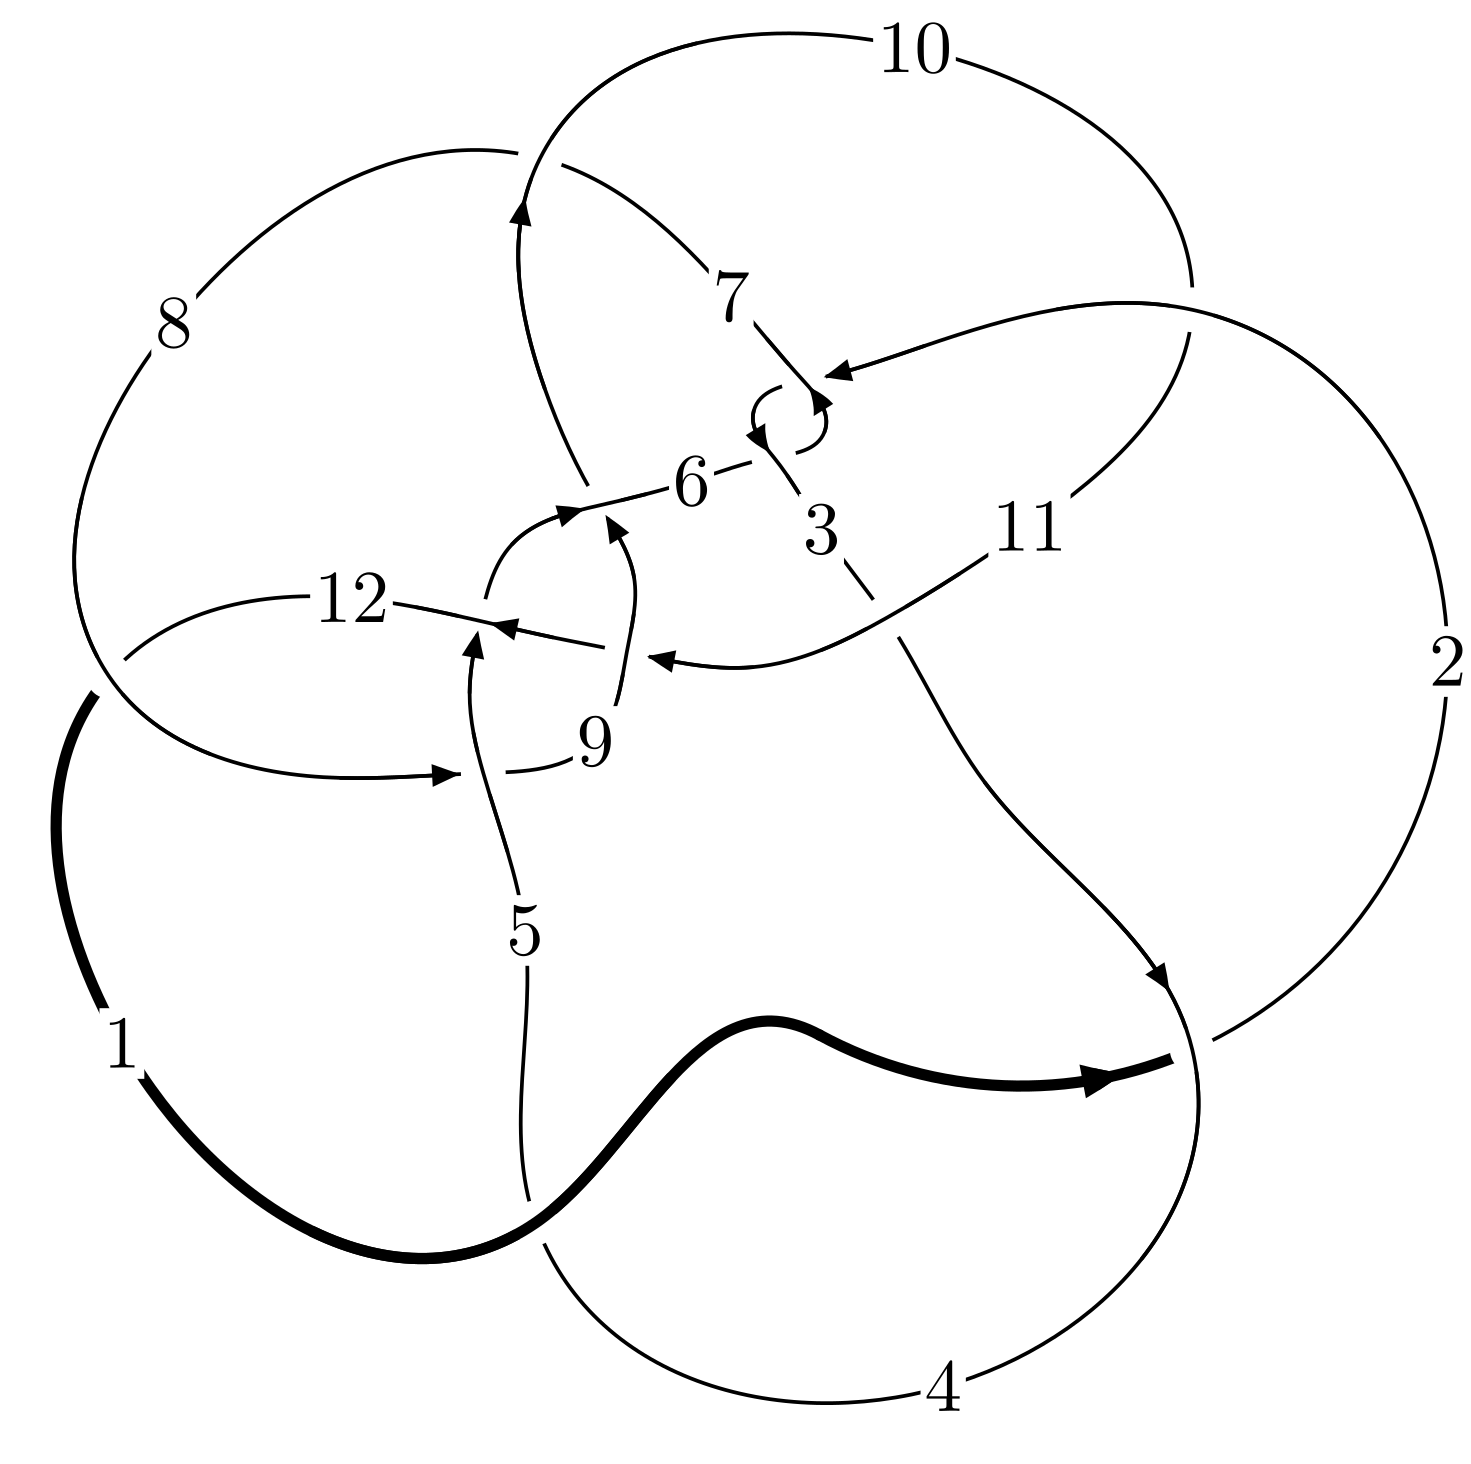
\includegraphics[width=112pt]{../../../GIT/diagram.site/Diagrams/png/1911_12a_1110.png}\\
\ \ \ A knot diagram\footnotemark}&
\allowdisplaybreaks
\textbf{Linearized knot diagam} \\
\cline{2-2}
 &
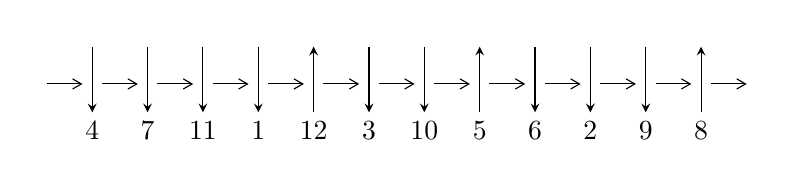
\begin{tikzpicture}[x=20pt, y=17pt]
	% nodes
	\node (C0) at (0, 0) {};
	\node (C1) at (1, 0) {};
	\node (C1U) at (1, +1) {};
	\node (C1D) at (1, -1) {4};

	\node (C2) at (2, 0) {};
	\node (C2U) at (2, +1) {};
	\node (C2D) at (2, -1) {7};

	\node (C3) at (3, 0) {};
	\node (C3U) at (3, +1) {};
	\node (C3D) at (3, -1) {11};

	\node (C4) at (4, 0) {};
	\node (C4U) at (4, +1) {};
	\node (C4D) at (4, -1) {1};

	\node (C5) at (5, 0) {};
	\node (C5U) at (5, +1) {};
	\node (C5D) at (5, -1) {12};

	\node (C6) at (6, 0) {};
	\node (C6U) at (6, +1) {};
	\node (C6D) at (6, -1) {3};

	\node (C7) at (7, 0) {};
	\node (C7U) at (7, +1) {};
	\node (C7D) at (7, -1) {10};

	\node (C8) at (8, 0) {};
	\node (C8U) at (8, +1) {};
	\node (C8D) at (8, -1) {5};

	\node (C9) at (9, 0) {};
	\node (C9U) at (9, +1) {};
	\node (C9D) at (9, -1) {6};

	\node (C10) at (10, 0) {};
	\node (C10U) at (10, +1) {};
	\node (C10D) at (10, -1) {2};

	\node (C11) at (11, 0) {};
	\node (C11U) at (11, +1) {};
	\node (C11D) at (11, -1) {9};

	\node (C12) at (12, 0) {};
	\node (C12U) at (12, +1) {};
	\node (C12D) at (12, -1) {8};
	\node (C13) at (13, 0) {};

	% arrows
	\draw[->,>={angle 60}]
	(C0) edge (C1) (C1) edge (C2) (C2) edge (C3) (C3) edge (C4) (C4) edge (C5) (C5) edge (C6) (C6) edge (C7) (C7) edge (C8) (C8) edge (C9) (C9) edge (C10) (C10) edge (C11) (C11) edge (C12) (C12) edge (C13) ;	\draw[->,>=stealth]
	(C1U) edge (C1D) (C2U) edge (C2D) (C3U) edge (C3D) (C4U) edge (C4D) (C5D) edge (C5U) (C6U) edge (C6D) (C7U) edge (C7D) (C8D) edge (C8U) (C9U) edge (C9D) (C10U) edge (C10D) (C11U) edge (C11D) (C12D) edge (C12U) ;
	\end{tikzpicture} \\
\hhline{~~} \\& 
\textbf{Solving Sequence} \\ \cline{2-2} 
 &
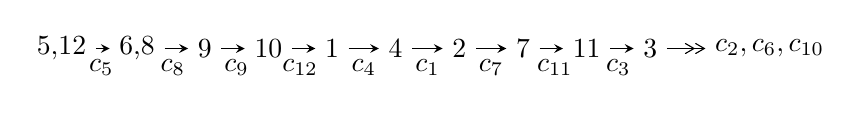
\begin{tikzpicture}[x=23pt, y=7pt]
	% node
	\node (A0) at (-1/8, 0) {5,12};
	\node (A1) at (17/16, 0) {6,8};
	\node (A2) at (17/8, 0) {9};
	\node (A3) at (25/8, 0) {10};
	\node (A4) at (33/8, 0) {1};
	\node (A5) at (41/8, 0) {4};
	\node (A6) at (49/8, 0) {2};
	\node (A7) at (57/8, 0) {7};
	\node (A8) at (65/8, 0) {11};
	\node (A9) at (73/8, 0) {3};
	\node (C1) at (1/2, -1) {$c_{5}$};
	\node (C2) at (13/8, -1) {$c_{8}$};
	\node (C3) at (21/8, -1) {$c_{9}$};
	\node (C4) at (29/8, -1) {$c_{12}$};
	\node (C5) at (37/8, -1) {$c_{4}$};
	\node (C6) at (45/8, -1) {$c_{1}$};
	\node (C7) at (53/8, -1) {$c_{7}$};
	\node (C8) at (61/8, -1) {$c_{11}$};
	\node (C9) at (69/8, -1) {$c_{3}$};
	\node (A10) at (11, 0) {$c_{2},c_{6},c_{10}$};

	% edge
	\draw[->,>=stealth]	
	(A0) edge (A1) (A1) edge (A2) (A2) edge (A3) (A3) edge (A4) (A4) edge (A5) (A5) edge (A6) (A6) edge (A7) (A7) edge (A8) (A8) edge (A9) ;
	\draw[->>,>={angle 60}]	
	(A9) edge (A10);
\end{tikzpicture} \\ 

\end{tabular} \\

\footnotetext{
The image of knot diagram is generated by the software ``\textbf{Draw programme}" developed by Andrew Bartholomew(\url{http://www.layer8.co.uk/maths/draw/index.htm\#Running-draw}), where we modified some parts for our purpose(\url{https://github.com/CATsTAILs/LinksPainter}).
}\phantom \\ \newline 
\centering \textbf{Ideals for irreducible components\footnotemark of $X_{\text{par}}$} 
 
\begin{align*}
I^u_{1}&=\langle 
-1.04121\times10^{1911} u^{192}-2.94515\times10^{1911} u^{191}+\cdots+4.61076\times10^{1912} b-7.76576\times10^{1911},\\
\phantom{I^u_{1}}&\phantom{= \langle  }-2.94044\times10^{1913} u^{192}-4.69682\times10^{1913} u^{191}+\cdots+5.48680\times10^{1914} a-2.38829\times10^{1916},\\
\phantom{I^u_{1}}&\phantom{= \langle  }u^{193}+3 u^{192}+\cdots+1523 u-119\rangle \\
I^u_{2}&=\langle 
-1.57865\times10^{116} u^{51}-2.29335\times10^{116} u^{50}+\cdots+9.68988\times10^{115} b-5.77826\times10^{116},\\
\phantom{I^u_{2}}&\phantom{= \langle  }-5.73748\times10^{116} u^{51}+3.04708\times10^{116} u^{50}+\cdots+9.68988\times10^{115} a+4.52810\times10^{116},\\
\phantom{I^u_{2}}&\phantom{= \langle  }u^{52}-4 u^{50}+\cdots-4 u+1\rangle \\
\\
\end{align*}
\raggedright * 2 irreducible components of $\dim_{\mathbb{C}}=0$, with total 245 representations.\\
\footnotetext{All coefficients of polynomials are rational numbers. But the coefficients are sometimes approximated in decimal forms when there is not enough margin.}
\newpage
\renewcommand{\arraystretch}{1}
\centering \section*{I. $I^u_{1}= \langle -1.04\times10^{1911} u^{192}-2.95\times10^{1911} u^{191}+\cdots+4.61\times10^{1912} b-7.77\times10^{1911},\;-2.94\times10^{1913} u^{192}-4.70\times10^{1913} u^{191}+\cdots+5.49\times10^{1914} a-2.39\times10^{1916},\;u^{193}+3 u^{192}+\cdots+1523 u-119 \rangle$}
\flushleft \textbf{(i) Arc colorings}\\
\begin{tabular}{m{7pt} m{180pt} m{7pt} m{180pt} }
\flushright $a_{5}=$&$\begin{pmatrix}1\\0\end{pmatrix}$ \\
\flushright $a_{12}=$&$\begin{pmatrix}0\\u\end{pmatrix}$ \\
\flushright $a_{6}=$&$\begin{pmatrix}1\\- u^2\end{pmatrix}$ \\
\flushright $a_{8}=$&$\begin{pmatrix}0.0535911 u^{192}+0.0856021 u^{191}+\cdots-543.246 u+43.5280\\0.0225821 u^{192}+0.0638757 u^{191}+\cdots-33.0712 u+0.168427\end{pmatrix}$ \\
\flushright $a_{9}=$&$\begin{pmatrix}0.0761733 u^{192}+0.149478 u^{191}+\cdots-576.317 u+43.6964\\0.0225821 u^{192}+0.0638757 u^{191}+\cdots-33.0712 u+0.168427\end{pmatrix}$ \\
\flushright $a_{10}=$&$\begin{pmatrix}0.0863457 u^{192}+0.169045 u^{191}+\cdots-672.692 u+52.9340\\0.0294198 u^{192}+0.0826882 u^{191}+\cdots-50.9591 u+1.47152\end{pmatrix}$ \\
\flushright $a_{1}=$&$\begin{pmatrix}0.0642413 u^{192}+0.291640 u^{191}+\cdots+836.760 u-76.0046\\-0.00576962 u^{192}-0.00872474 u^{191}+\cdots+45.0307 u-3.65749\end{pmatrix}$ \\
\flushright $a_{4}=$&$\begin{pmatrix}0.412073 u^{192}+1.23966 u^{191}+\cdots-977.632 u+59.6963\\-0.0178693 u^{192}-0.0567235 u^{191}+\cdots+63.3657 u-5.88625\end{pmatrix}$ \\
\flushright $a_{2}=$&$\begin{pmatrix}-0.165086 u^{192}-0.670371 u^{191}+\cdots-693.144 u+70.2498\\0.0165588 u^{192}+0.0422727 u^{191}+\cdots-94.7746 u+5.91355\end{pmatrix}$ \\
\flushright $a_{7}=$&$\begin{pmatrix}-0.255540 u^{192}-0.816600 u^{191}+\cdots+132.364 u+1.18893\\-0.0165383 u^{192}-0.0395895 u^{191}+\cdots+89.7596 u-8.46992\end{pmatrix}$ \\
\flushright $a_{11}=$&$\begin{pmatrix}0.0793911 u^{192}+0.335477 u^{191}+\cdots+762.122 u-70.3606\\0.0209194 u^{192}+0.0525618 u^{191}+\cdots-117.668 u+9.30155\end{pmatrix}$ \\
\flushright $a_{3}=$&$\begin{pmatrix}-0.00837962 u^{192}+0.0846030 u^{191}+\cdots+909.256 u-84.1823\\-0.0173126 u^{192}-0.0527161 u^{191}+\cdots+57.7225 u-4.57325\end{pmatrix}$\\&\end{tabular}
\flushleft \textbf{(ii) Obstruction class $= -1$}\\~\\
\flushleft \textbf{(iii) Cusp Shapes $= -0.491202 u^{192}-1.60985 u^{191}+\cdots-92.7171 u+27.7140$}\\~\\
\newpage\renewcommand{\arraystretch}{1}
\flushleft \textbf{(iv) u-Polynomials at the component}\newline \\
\begin{tabular}{m{50pt}|m{274pt}}
Crossings & \hspace{64pt}u-Polynomials at each crossing \\
\hline $$\begin{aligned}c_{1},c_{4}\end{aligned}$$&$\begin{aligned}
&u^{193}-9 u^{192}+\cdots-25294392 u+821143
\end{aligned}$\\
\hline $$\begin{aligned}c_{2},c_{6}\end{aligned}$$&$\begin{aligned}
&u^{193}+3 u^{192}+\cdots-9488 u+1279
\end{aligned}$\\
\hline $$\begin{aligned}c_{3}\end{aligned}$$&$\begin{aligned}
&u^{193}- u^{192}+\cdots-84164118 u+75604697
\end{aligned}$\\
\hline $$\begin{aligned}c_{5}\end{aligned}$$&$\begin{aligned}
&u^{193}-3 u^{192}+\cdots+1523 u+119
\end{aligned}$\\
\hline $$\begin{aligned}c_{7}\end{aligned}$$&$\begin{aligned}
&u^{193}+4 u^{192}+\cdots-136105380 u+161762888
\end{aligned}$\\
\hline $$\begin{aligned}c_{8}\end{aligned}$$&$\begin{aligned}
&u^{193}-4 u^{192}+\cdots+66807 u+16531
\end{aligned}$\\
\hline $$\begin{aligned}c_{9}\end{aligned}$$&$\begin{aligned}
&u^{193}+2 u^{192}+\cdots-19697810 u+389851
\end{aligned}$\\
\hline $$\begin{aligned}c_{10}\end{aligned}$$&$\begin{aligned}
&u^{193}-5 u^{192}+\cdots-885248946 u+70940957
\end{aligned}$\\
\hline $$\begin{aligned}c_{11}\end{aligned}$$&$\begin{aligned}
&u^{193}+6 u^{192}+\cdots-3800155 u+329741
\end{aligned}$\\
\hline $$\begin{aligned}c_{12}\end{aligned}$$&$\begin{aligned}
&u^{193}-24 u^{191}+\cdots+71854 u+6323
\end{aligned}$\\
\hline
\end{tabular}\\~\\
\newpage\renewcommand{\arraystretch}{1}
\flushleft \textbf{(v) Riley Polynomials at the component}\newline \\
\begin{tabular}{m{50pt}|m{274pt}}
Crossings & \hspace{64pt}Riley Polynomials at each crossing \\
\hline $$\begin{aligned}c_{1},c_{4}\end{aligned}$$&$\begin{aligned}
&y^{193}+149 y^{192}+\cdots+91423314119834 y-674275826449
\end{aligned}$\\
\hline $$\begin{aligned}c_{2},c_{6}\end{aligned}$$&$\begin{aligned}
&y^{193}+115 y^{192}+\cdots+62705262 y-1635841
\end{aligned}$\\
\hline $$\begin{aligned}c_{3}\end{aligned}$$&$\begin{aligned}
&y^{193}+81 y^{192}+\cdots-246539706104330476 y-5716070208461809
\end{aligned}$\\
\hline $$\begin{aligned}c_{5}\end{aligned}$$&$\begin{aligned}
&y^{193}+7 y^{192}+\cdots-804935 y-14161
\end{aligned}$\\
\hline $$\begin{aligned}c_{7}\end{aligned}$$&$\begin{aligned}
&y^{193}+22 y^{192}+\cdots+1403258281552618544 y-26167231934100544
\end{aligned}$\\
\hline $$\begin{aligned}c_{8}\end{aligned}$$&$\begin{aligned}
&y^{193}-46 y^{192}+\cdots+29373639963 y-273273961
\end{aligned}$\\
\hline $$\begin{aligned}c_{9}\end{aligned}$$&$\begin{aligned}
&y^{193}-48 y^{192}+\cdots+204957052058088 y-151983802201
\end{aligned}$\\
\hline $$\begin{aligned}c_{10}\end{aligned}$$&$\begin{aligned}
&y^{193}+71 y^{192}+\cdots-122129491189476726 y-5032619380075849
\end{aligned}$\\
\hline $$\begin{aligned}c_{11}\end{aligned}$$&$\begin{aligned}
&y^{193}+86 y^{191}+\cdots-7760857914797 y-108729127081
\end{aligned}$\\
\hline $$\begin{aligned}c_{12}\end{aligned}$$&$\begin{aligned}
&y^{193}-48 y^{192}+\cdots+3821977538 y-39980329
\end{aligned}$\\
\hline
\end{tabular}\\~\\
\newpage\flushleft \textbf{(vi) Complex Volumes and Cusp Shapes}
$$\begin{array}{c|c|c}  
\text{Solutions to }I^u_{1}& \I (\text{vol} + \sqrt{-1}CS) & \text{Cusp shape}\\
 \hline 
\begin{aligned}
u &= \phantom{-}0.497238 + 0.867067 I \\
a &= \phantom{-}0.342922 + 0.745631 I \\
b &= \phantom{-}0.766058 - 0.204781 I\end{aligned}
 & \phantom{-}4.22094 - 3.31943 I & \phantom{-0.000000 } 0 \\ \hline\begin{aligned}
u &= \phantom{-}0.497238 - 0.867067 I \\
a &= \phantom{-}0.342922 - 0.745631 I \\
b &= \phantom{-}0.766058 + 0.204781 I\end{aligned}
 & \phantom{-}4.22094 + 3.31943 I & \phantom{-0.000000 } 0 \\ \hline\begin{aligned}
u &= -1.002190 + 0.090826 I \\
a &= \phantom{-}1.26913 - 0.92294 I \\
b &= -1.002540 + 0.366203 I\end{aligned}
 & \phantom{-}7.64125 - 4.06324 I & \phantom{-0.000000 } 0 \\ \hline\begin{aligned}
u &= -1.002190 - 0.090826 I \\
a &= \phantom{-}1.26913 + 0.92294 I \\
b &= -1.002540 - 0.366203 I\end{aligned}
 & \phantom{-}7.64125 + 4.06324 I & \phantom{-0.000000 } 0 \\ \hline\begin{aligned}
u &= -0.523190 + 0.839731 I \\
a &= \phantom{-}0.611273 - 0.989258 I \\
b &= \phantom{-}0.438938 - 0.201154 I\end{aligned}
 & \phantom{-}2.63803 - 4.74363 I & \phantom{-0.000000 } 0 \\ \hline\begin{aligned}
u &= -0.523190 - 0.839731 I \\
a &= \phantom{-}0.611273 + 0.989258 I \\
b &= \phantom{-}0.438938 + 0.201154 I\end{aligned}
 & \phantom{-}2.63803 + 4.74363 I & \phantom{-0.000000 } 0 \\ \hline\begin{aligned}
u &= \phantom{-}0.886144 + 0.508299 I \\
a &= -0.821468 + 0.607193 I \\
b &= \phantom{-}0.881728 + 0.546357 I\end{aligned}
 & \phantom{-}6.25595 - 0.94873 I & \phantom{-0.000000 } 0 \\ \hline\begin{aligned}
u &= \phantom{-}0.886144 - 0.508299 I \\
a &= -0.821468 - 0.607193 I \\
b &= \phantom{-}0.881728 - 0.546357 I\end{aligned}
 & \phantom{-}6.25595 + 0.94873 I & \phantom{-0.000000 } 0 \\ \hline\begin{aligned}
u &= -0.793213 + 0.557530 I \\
a &= \phantom{-}0.974293 + 0.051565 I \\
b &= -0.794389 + 0.462012 I\end{aligned}
 & \phantom{-}1.25526 - 1.43426 I & \phantom{-0.000000 } 0 \\ \hline\begin{aligned}
u &= -0.793213 - 0.557530 I \\
a &= \phantom{-}0.974293 - 0.051565 I \\
b &= -0.794389 - 0.462012 I\end{aligned}
 & \phantom{-}1.25526 + 1.43426 I & \phantom{-0.000000 } 0\\
 \hline 
 \end{array}$$\newpage$$\begin{array}{c|c|c}  
\text{Solutions to }I^u_{1}& \I (\text{vol} + \sqrt{-1}CS) & \text{Cusp shape}\\
 \hline 
\begin{aligned}
u &= \phantom{-}0.782743 + 0.569579 I \\
a &= \phantom{-}1.274100 + 0.182530 I \\
b &= -1.38722 - 1.02429 I\end{aligned}
 & \phantom{-}5.57186 + 7.41914 I & \phantom{-0.000000 } 0 \\ \hline\begin{aligned}
u &= \phantom{-}0.782743 - 0.569579 I \\
a &= \phantom{-}1.274100 - 0.182530 I \\
b &= -1.38722 + 1.02429 I\end{aligned}
 & \phantom{-}5.57186 - 7.41914 I & \phantom{-0.000000 } 0 \\ \hline\begin{aligned}
u &= -0.851088 + 0.458366 I \\
a &= \phantom{-}1.49827 + 0.77108 I \\
b &= -0.736769 + 0.465369 I\end{aligned}
 & \phantom{-}0.74560 - 2.43904 I & \phantom{-0.000000 } 0 \\ \hline\begin{aligned}
u &= -0.851088 - 0.458366 I \\
a &= \phantom{-}1.49827 - 0.77108 I \\
b &= -0.736769 - 0.465369 I\end{aligned}
 & \phantom{-}0.74560 + 2.43904 I & \phantom{-0.000000 } 0 \\ \hline\begin{aligned}
u &= \phantom{-}0.779871 + 0.529450 I \\
a &= -1.13842 + 1.20231 I \\
b &= \phantom{-}0.660187 + 0.567217 I\end{aligned}
 & \phantom{-}3.48058 + 8.67580 I & \phantom{-0.000000 } 0 \\ \hline\begin{aligned}
u &= \phantom{-}0.779871 - 0.529450 I \\
a &= -1.13842 - 1.20231 I \\
b &= \phantom{-}0.660187 - 0.567217 I\end{aligned}
 & \phantom{-}3.48058 - 8.67580 I & \phantom{-0.000000 } 0 \\ \hline\begin{aligned}
u &= \phantom{-}0.453131 + 0.806446 I \\
a &= -0.297623 + 0.200067 I \\
b &= \phantom{-}0.440139 - 1.248480 I\end{aligned}
 & \phantom{-}0.183860 + 0.947346 I & \phantom{-0.000000 } 0 \\ \hline\begin{aligned}
u &= \phantom{-}0.453131 - 0.806446 I \\
a &= -0.297623 - 0.200067 I \\
b &= \phantom{-}0.440139 + 1.248480 I\end{aligned}
 & \phantom{-}0.183860 - 0.947346 I & \phantom{-0.000000 } 0 \\ \hline\begin{aligned}
u &= -0.630913 + 0.672528 I \\
a &= \phantom{-}1.84382 + 0.30274 I \\
b &= -0.945622 + 0.822813 I\end{aligned}
 & \phantom{-}7.03056 - 3.49193 I & \phantom{-0.000000 } 0 \\ \hline\begin{aligned}
u &= -0.630913 - 0.672528 I \\
a &= \phantom{-}1.84382 - 0.30274 I \\
b &= -0.945622 - 0.822813 I\end{aligned}
 & \phantom{-}7.03056 + 3.49193 I & \phantom{-0.000000 } 0\\
 \hline 
 \end{array}$$\newpage$$\begin{array}{c|c|c}  
\text{Solutions to }I^u_{1}& \I (\text{vol} + \sqrt{-1}CS) & \text{Cusp shape}\\
 \hline 
\begin{aligned}
u &= \phantom{-}0.776522 + 0.752682 I \\
a &= -1.299440 + 0.428593 I \\
b &= \phantom{-}1.13141 + 1.06210 I\end{aligned}
 & \phantom{-}8.60089 + 7.20452 I & \phantom{-0.000000 } 0 \\ \hline\begin{aligned}
u &= \phantom{-}0.776522 - 0.752682 I \\
a &= -1.299440 - 0.428593 I \\
b &= \phantom{-}1.13141 - 1.06210 I\end{aligned}
 & \phantom{-}8.60089 - 7.20452 I & \phantom{-0.000000 } 0 \\ \hline\begin{aligned}
u &= \phantom{-}0.195212 + 0.888065 I \\
a &= -0.715216 - 0.818022 I \\
b &= \phantom{-}0.011872 - 0.684290 I\end{aligned}
 & -1.77741 + 2.64700 I & \phantom{-0.000000 } 0 \\ \hline\begin{aligned}
u &= \phantom{-}0.195212 - 0.888065 I \\
a &= -0.715216 + 0.818022 I \\
b &= \phantom{-}0.011872 + 0.684290 I\end{aligned}
 & -1.77741 - 2.64700 I & \phantom{-0.000000 } 0 \\ \hline\begin{aligned}
u &= -0.790986 + 0.753719 I \\
a &= \phantom{-}1.217110 + 0.188763 I \\
b &= -1.32910 + 0.93706 I\end{aligned}
 & \phantom{-}6.07885 - 2.57363 I & \phantom{-0.000000 } 0 \\ \hline\begin{aligned}
u &= -0.790986 - 0.753719 I \\
a &= \phantom{-}1.217110 - 0.188763 I \\
b &= -1.32910 - 0.93706 I\end{aligned}
 & \phantom{-}6.07885 + 2.57363 I & \phantom{-0.000000 } 0 \\ \hline\begin{aligned}
u &= \phantom{-}0.797521 + 0.752341 I \\
a &= -1.059590 + 0.244506 I \\
b &= \phantom{-}1.44584 + 1.10749 I\end{aligned}
 & \phantom{-}9.93565 - 1.33558 I & \phantom{-0.000000 } 0 \\ \hline\begin{aligned}
u &= \phantom{-}0.797521 - 0.752341 I \\
a &= -1.059590 - 0.244506 I \\
b &= \phantom{-}1.44584 - 1.10749 I\end{aligned}
 & \phantom{-}9.93565 + 1.33558 I & \phantom{-0.000000 } 0 \\ \hline\begin{aligned}
u &= -0.951939 + 0.544515 I \\
a &= \phantom{-}0.489202 + 0.357652 I \\
b &= -1.123300 - 0.502790 I\end{aligned}
 & \phantom{-}2.50050 + 1.59976 I & \phantom{-0.000000 } 0 \\ \hline\begin{aligned}
u &= -0.951939 - 0.544515 I \\
a &= \phantom{-}0.489202 - 0.357652 I \\
b &= -1.123300 + 0.502790 I\end{aligned}
 & \phantom{-}2.50050 - 1.59976 I & \phantom{-0.000000 } 0\\
 \hline 
 \end{array}$$\newpage$$\begin{array}{c|c|c}  
\text{Solutions to }I^u_{1}& \I (\text{vol} + \sqrt{-1}CS) & \text{Cusp shape}\\
 \hline 
\begin{aligned}
u &= \phantom{-}0.126973 + 0.893867 I \\
a &= -0.077761 + 0.155141 I \\
b &= \phantom{-}0.02011 - 1.78711 I\end{aligned}
 & -0.49385 + 1.44634 I & \phantom{-0.000000 } 0 \\ \hline\begin{aligned}
u &= \phantom{-}0.126973 - 0.893867 I \\
a &= -0.077761 - 0.155141 I \\
b &= \phantom{-}0.02011 + 1.78711 I\end{aligned}
 & -0.49385 - 1.44634 I & \phantom{-0.000000 } 0 \\ \hline\begin{aligned}
u &= -0.007647 + 1.106220 I \\
a &= \phantom{-}0.743541 - 0.075769 I \\
b &= -0.949225 + 0.668062 I\end{aligned}
 & \phantom{-}0.63290 - 4.78567 I & \phantom{-0.000000 } 0 \\ \hline\begin{aligned}
u &= -0.007647 - 1.106220 I \\
a &= \phantom{-}0.743541 + 0.075769 I \\
b &= -0.949225 - 0.668062 I\end{aligned}
 & \phantom{-}0.63290 + 4.78567 I & \phantom{-0.000000 } 0 \\ \hline\begin{aligned}
u &= -0.853441 + 0.260269 I \\
a &= -1.147830 + 0.526623 I \\
b &= \phantom{-}1.26617 - 1.05813 I\end{aligned}
 & \phantom{-}8.51652 - 1.44069 I & \phantom{-0.000000 } 0 \\ \hline\begin{aligned}
u &= -0.853441 - 0.260269 I \\
a &= -1.147830 - 0.526623 I \\
b &= \phantom{-}1.26617 + 1.05813 I\end{aligned}
 & \phantom{-}8.51652 + 1.44069 I & \phantom{-0.000000 } 0 \\ \hline\begin{aligned}
u &= -0.876499 + 0.061956 I \\
a &= \phantom{-}0.573900 + 0.422916 I \\
b &= -0.930012 - 0.080698 I\end{aligned}
 & \phantom{-}2.16628 + 1.75332 I & \phantom{-0.000000 } 0 \\ \hline\begin{aligned}
u &= -0.876499 - 0.061956 I \\
a &= \phantom{-}0.573900 - 0.422916 I \\
b &= -0.930012 + 0.080698 I\end{aligned}
 & \phantom{-}2.16628 - 1.75332 I & \phantom{-0.000000 } 0 \\ \hline\begin{aligned}
u &= \phantom{-}0.165929 + 0.848786 I \\
a &= -1.41513 - 0.11976 I \\
b &= \phantom{-}1.58164 + 0.24148 I\end{aligned}
 & -0.67690 + 2.98996 I & \phantom{-0.000000 } 0 \\ \hline\begin{aligned}
u &= \phantom{-}0.165929 - 0.848786 I \\
a &= -1.41513 + 0.11976 I \\
b &= \phantom{-}1.58164 - 0.24148 I\end{aligned}
 & -0.67690 - 2.98996 I & \phantom{-0.000000 } 0\\
 \hline 
 \end{array}$$\newpage$$\begin{array}{c|c|c}  
\text{Solutions to }I^u_{1}& \I (\text{vol} + \sqrt{-1}CS) & \text{Cusp shape}\\
 \hline 
\begin{aligned}
u &= \phantom{-}0.803737 + 0.317029 I \\
a &= -1.49987 + 2.33986 I \\
b &= \phantom{-}0.575461 - 0.082402 I\end{aligned}
 & \phantom{-}7.26083 + 11.03510 I & \phantom{-0.000000 } 0 \\ \hline\begin{aligned}
u &= \phantom{-}0.803737 - 0.317029 I \\
a &= -1.49987 - 2.33986 I \\
b &= \phantom{-}0.575461 + 0.082402 I\end{aligned}
 & \phantom{-}7.26083 - 11.03510 I & \phantom{-0.000000 } 0 \\ \hline\begin{aligned}
u &= \phantom{-}0.649043 + 0.952767 I \\
a &= \phantom{-}0.781237 - 0.141581 I \\
b &= -0.901277 - 0.981986 I\end{aligned}
 & -1.77817 + 4.15644 I & \phantom{-0.000000 } 0 \\ \hline\begin{aligned}
u &= \phantom{-}0.649043 - 0.952767 I \\
a &= \phantom{-}0.781237 + 0.141581 I \\
b &= -0.901277 + 0.981986 I\end{aligned}
 & -1.77817 - 4.15644 I & \phantom{-0.000000 } 0 \\ \hline\begin{aligned}
u &= \phantom{-}0.573211 + 0.620217 I \\
a &= -0.37608 - 2.05342 I \\
b &= -0.414764 + 0.050057 I\end{aligned}
 & \phantom{-}0.994026 + 0.137447 I & \phantom{-0.000000 } 0 \\ \hline\begin{aligned}
u &= \phantom{-}0.573211 - 0.620217 I \\
a &= -0.37608 + 2.05342 I \\
b &= -0.414764 - 0.050057 I\end{aligned}
 & \phantom{-}0.994026 - 0.137447 I & \phantom{-0.000000 } 0 \\ \hline\begin{aligned}
u &= \phantom{-}0.921411 + 0.713068 I \\
a &= \phantom{-}1.64042 - 0.40033 I \\
b &= -0.724146 - 0.731262 I\end{aligned}
 & \phantom{-}1.19042 + 3.64605 I & \phantom{-0.000000 } 0 \\ \hline\begin{aligned}
u &= \phantom{-}0.921411 - 0.713068 I \\
a &= \phantom{-}1.64042 + 0.40033 I \\
b &= -0.724146 + 0.731262 I\end{aligned}
 & \phantom{-}1.19042 - 3.64605 I & \phantom{-0.000000 } 0 \\ \hline\begin{aligned}
u &= -0.825514 + 0.123471 I \\
a &= \phantom{-}2.31676 + 1.77210 I \\
b &= -0.596108 - 0.196613 I\end{aligned}
 & \phantom{-}3.81726 - 4.73968 I & \phantom{-0.000000 } 0 \\ \hline\begin{aligned}
u &= -0.825514 - 0.123471 I \\
a &= \phantom{-}2.31676 - 1.77210 I \\
b &= -0.596108 + 0.196613 I\end{aligned}
 & \phantom{-}3.81726 + 4.73968 I & \phantom{-0.000000 } 0\\
 \hline 
 \end{array}$$\newpage$$\begin{array}{c|c|c}  
\text{Solutions to }I^u_{1}& \I (\text{vol} + \sqrt{-1}CS) & \text{Cusp shape}\\
 \hline 
\begin{aligned}
u &= \phantom{-}0.139188 + 0.816122 I \\
a &= \phantom{-}0.937503 - 0.580994 I \\
b &= -0.077951 - 0.659096 I\end{aligned}
 & -2.19429 - 0.01698 I & \phantom{-0.000000 } 0 \\ \hline\begin{aligned}
u &= \phantom{-}0.139188 - 0.816122 I \\
a &= \phantom{-}0.937503 + 0.580994 I \\
b &= -0.077951 + 0.659096 I\end{aligned}
 & -2.19429 + 0.01698 I & \phantom{-0.000000 } 0 \\ \hline\begin{aligned}
u &= \phantom{-}1.171430 + 0.072628 I \\
a &= -1.52428 + 0.87247 I \\
b &= \phantom{-}0.785423 - 0.206755 I\end{aligned}
 & \phantom{-}9.81622 - 0.34797 I & \phantom{-0.000000 } 0 \\ \hline\begin{aligned}
u &= \phantom{-}1.171430 - 0.072628 I \\
a &= -1.52428 - 0.87247 I \\
b &= \phantom{-}0.785423 + 0.206755 I\end{aligned}
 & \phantom{-}9.81622 + 0.34797 I & \phantom{-0.000000 } 0 \\ \hline\begin{aligned}
u &= -0.133692 + 1.175910 I \\
a &= \phantom{-}1.312150 + 0.015195 I \\
b &= -1.49715 + 0.23346 I\end{aligned}
 & \phantom{-}3.01136 - 7.70054 I & \phantom{-0.000000 } 0 \\ \hline\begin{aligned}
u &= -0.133692 - 1.175910 I \\
a &= \phantom{-}1.312150 - 0.015195 I \\
b &= -1.49715 - 0.23346 I\end{aligned}
 & \phantom{-}3.01136 + 7.70054 I & \phantom{-0.000000 } 0 \\ \hline\begin{aligned}
u &= \phantom{-}0.441030 + 1.099470 I \\
a &= \phantom{-}0.116560 - 0.489882 I \\
b &= -0.951543 + 0.580989 I\end{aligned}
 & \phantom{-}7.47534 - 2.11083 I & \phantom{-0.000000 } 0 \\ \hline\begin{aligned}
u &= \phantom{-}0.441030 - 1.099470 I \\
a &= \phantom{-}0.116560 + 0.489882 I \\
b &= -0.951543 - 0.580989 I\end{aligned}
 & \phantom{-}7.47534 + 2.11083 I & \phantom{-0.000000 } 0 \\ \hline\begin{aligned}
u &= -0.463152 + 1.094350 I \\
a &= \phantom{-}0.027504 - 0.529615 I \\
b &= \phantom{-}0.898045 + 0.196218 I\end{aligned}
 & \phantom{-}5.01813 - 2.63269 I & \phantom{-0.000000 } 0 \\ \hline\begin{aligned}
u &= -0.463152 - 1.094350 I \\
a &= \phantom{-}0.027504 + 0.529615 I \\
b &= \phantom{-}0.898045 - 0.196218 I\end{aligned}
 & \phantom{-}5.01813 + 2.63269 I & \phantom{-0.000000 } 0\\
 \hline 
 \end{array}$$\newpage$$\begin{array}{c|c|c}  
\text{Solutions to }I^u_{1}& \I (\text{vol} + \sqrt{-1}CS) & \text{Cusp shape}\\
 \hline 
\begin{aligned}
u &= \phantom{-}0.088256 + 0.806160 I \\
a &= -0.708291 - 0.331551 I \\
b &= \phantom{-}0.727895 + 0.928715 I\end{aligned}
 & -2.45003 - 0.79596 I & \phantom{-0.000000 } 0 \\ \hline\begin{aligned}
u &= \phantom{-}0.088256 - 0.806160 I \\
a &= -0.708291 + 0.331551 I \\
b &= \phantom{-}0.727895 - 0.928715 I\end{aligned}
 & -2.45003 + 0.79596 I & \phantom{-0.000000 } 0 \\ \hline\begin{aligned}
u &= \phantom{-}0.450658 + 1.101640 I \\
a &= -0.032820 - 0.395267 I \\
b &= -1.216170 + 0.126684 I\end{aligned}
 & \phantom{-}8.87783 + 6.48175 I & \phantom{-0.000000 } 0 \\ \hline\begin{aligned}
u &= \phantom{-}0.450658 - 1.101640 I \\
a &= -0.032820 + 0.395267 I \\
b &= -1.216170 - 0.126684 I\end{aligned}
 & \phantom{-}8.87783 - 6.48175 I & \phantom{-0.000000 } 0 \\ \hline\begin{aligned}
u &= -0.572026 + 1.061560 I \\
a &= \phantom{-}0.575727 - 0.252604 I \\
b &= \phantom{-}0.044850 - 0.309132 I\end{aligned}
 & \phantom{-}2.71678 - 4.55421 I & \phantom{-0.000000 } 0 \\ \hline\begin{aligned}
u &= -0.572026 - 1.061560 I \\
a &= \phantom{-}0.575727 + 0.252604 I \\
b &= \phantom{-}0.044850 + 0.309132 I\end{aligned}
 & \phantom{-}2.71678 + 4.55421 I & \phantom{-0.000000 } 0 \\ \hline\begin{aligned}
u &= \phantom{-}0.384659 + 0.690356 I \\
a &= \phantom{-}0.549022 - 0.287216 I \\
b &= -0.62026 + 1.81306 I\end{aligned}
 & \phantom{-}5.00288 + 12.48190 I & \phantom{-0.000000 } 0 \\ \hline\begin{aligned}
u &= \phantom{-}0.384659 - 0.690356 I \\
a &= \phantom{-}0.549022 + 0.287216 I \\
b &= -0.62026 - 1.81306 I\end{aligned}
 & \phantom{-}5.00288 - 12.48190 I & \phantom{-0.000000 } 0 \\ \hline\begin{aligned}
u &= -0.189988 + 0.766916 I \\
a &= \phantom{-}1.83626 + 0.68218 I \\
b &= -0.350538 + 0.601281 I\end{aligned}
 & \phantom{-}0.08290 - 7.67658 I & \phantom{-0.000000 } 0 \\ \hline\begin{aligned}
u &= -0.189988 - 0.766916 I \\
a &= \phantom{-}1.83626 - 0.68218 I \\
b &= -0.350538 - 0.601281 I\end{aligned}
 & \phantom{-}0.08290 + 7.67658 I & \phantom{-0.000000 } 0\\
 \hline 
 \end{array}$$\newpage$$\begin{array}{c|c|c}  
\text{Solutions to }I^u_{1}& \I (\text{vol} + \sqrt{-1}CS) & \text{Cusp shape}\\
 \hline 
\begin{aligned}
u &= -0.509411 + 0.594685 I \\
a &= \phantom{-}1.086050 - 0.284729 I \\
b &= -1.88307 + 0.40041 I\end{aligned}
 & \phantom{-}3.15731 + 0.59915 I & \phantom{-0.000000 } 0 \\ \hline\begin{aligned}
u &= -0.509411 - 0.594685 I \\
a &= \phantom{-}1.086050 + 0.284729 I \\
b &= -1.88307 - 0.40041 I\end{aligned}
 & \phantom{-}3.15731 - 0.59915 I & \phantom{-0.000000 } 0 \\ \hline\begin{aligned}
u &= -1.028350 + 0.656856 I \\
a &= -1.043240 + 0.144329 I \\
b &= \phantom{-}1.39115 - 0.98329 I\end{aligned}
 & \phantom{-}10.4059 - 11.6137 I & \phantom{-0.000000 } 0 \\ \hline\begin{aligned}
u &= -1.028350 - 0.656856 I \\
a &= -1.043240 - 0.144329 I \\
b &= \phantom{-}1.39115 + 0.98329 I\end{aligned}
 & \phantom{-}10.4059 + 11.6137 I & \phantom{-0.000000 } 0 \\ \hline\begin{aligned}
u &= -0.318620 + 0.706869 I \\
a &= -0.555493 - 0.359034 I \\
b &= \phantom{-}0.56663 + 1.67029 I\end{aligned}
 & \phantom{-}1.39988 - 6.81659 I & \phantom{-0.000000 } 0 \\ \hline\begin{aligned}
u &= -0.318620 - 0.706869 I \\
a &= -0.555493 + 0.359034 I \\
b &= \phantom{-}0.56663 - 1.67029 I\end{aligned}
 & \phantom{-}1.39988 + 6.81659 I & \phantom{-0.000000 } 0 \\ \hline\begin{aligned}
u &= \phantom{-}0.660774 + 1.056300 I \\
a &= \phantom{-}1.132000 - 0.208741 I \\
b &= -1.44104 - 0.96969 I\end{aligned}
 & \phantom{-}3.55642 + 7.82089 I & \phantom{-0.000000 } 0 \\ \hline\begin{aligned}
u &= \phantom{-}0.660774 - 1.056300 I \\
a &= \phantom{-}1.132000 + 0.208741 I \\
b &= -1.44104 + 0.96969 I\end{aligned}
 & \phantom{-}3.55642 - 7.82089 I & \phantom{-0.000000 } 0 \\ \hline\begin{aligned}
u &= \phantom{-}1.088800 + 0.625231 I \\
a &= -1.269830 - 0.279353 I \\
b &= \phantom{-}1.214680 + 0.561620 I\end{aligned}
 & \phantom{-}7.50739 + 4.54303 I & \phantom{-0.000000 } 0 \\ \hline\begin{aligned}
u &= \phantom{-}1.088800 - 0.625231 I \\
a &= -1.269830 + 0.279353 I \\
b &= \phantom{-}1.214680 - 0.561620 I\end{aligned}
 & \phantom{-}7.50739 - 4.54303 I & \phantom{-0.000000 } 0\\
 \hline 
 \end{array}$$\newpage$$\begin{array}{c|c|c}  
\text{Solutions to }I^u_{1}& \I (\text{vol} + \sqrt{-1}CS) & \text{Cusp shape}\\
 \hline 
\begin{aligned}
u &= -0.459806 + 1.178840 I \\
a &= \phantom{-}0.287699 - 0.074862 I \\
b &= \phantom{-}0.352696 - 0.647795 I\end{aligned}
 & \phantom{-}2.64925 - 4.48301 I & \phantom{-0.000000 } 0 \\ \hline\begin{aligned}
u &= -0.459806 - 1.178840 I \\
a &= \phantom{-}0.287699 + 0.074862 I \\
b &= \phantom{-}0.352696 + 0.647795 I\end{aligned}
 & \phantom{-}2.64925 + 4.48301 I & \phantom{-0.000000 } 0 \\ \hline\begin{aligned}
u &= \phantom{-}1.180090 + 0.481702 I \\
a &= -0.646109 - 0.202589 I \\
b &= \phantom{-}0.994019 + 0.448982 I\end{aligned}
 & \phantom{-}2.05102 + 1.14955 I & \phantom{-0.000000 } 0 \\ \hline\begin{aligned}
u &= \phantom{-}1.180090 - 0.481702 I \\
a &= -0.646109 + 0.202589 I \\
b &= \phantom{-}0.994019 - 0.448982 I\end{aligned}
 & \phantom{-}2.05102 - 1.14955 I & \phantom{-0.000000 } 0 \\ \hline\begin{aligned}
u &= -0.810075 + 1.005450 I \\
a &= \phantom{-}1.132610 + 0.087829 I \\
b &= -0.845222 + 0.747687 I\end{aligned}
 & \phantom{-}0.335352 - 0.698527 I & \phantom{-0.000000 } 0 \\ \hline\begin{aligned}
u &= -0.810075 - 1.005450 I \\
a &= \phantom{-}1.132610 - 0.087829 I \\
b &= -0.845222 - 0.747687 I\end{aligned}
 & \phantom{-}0.335352 + 0.698527 I & \phantom{-0.000000 } 0 \\ \hline\begin{aligned}
u &= \phantom{-}0.113438 + 0.679220 I \\
a &= \phantom{-}0.39029 - 2.28438 I \\
b &= -0.049904 - 1.157790 I\end{aligned}
 & -0.39576 + 1.86685 I & \phantom{-0.000000 } 0 \\ \hline\begin{aligned}
u &= \phantom{-}0.113438 - 0.679220 I \\
a &= \phantom{-}0.39029 + 2.28438 I \\
b &= -0.049904 + 1.157790 I\end{aligned}
 & -0.39576 - 1.86685 I & \phantom{-0.000000 } 0 \\ \hline\begin{aligned}
u &= \phantom{-}0.270853 + 0.630701 I \\
a &= \phantom{-}1.192930 - 0.324289 I \\
b &= -0.824645 - 1.084070 I\end{aligned}
 & -1.89359 + 3.29036 I & \phantom{-0.000000 } 0 \\ \hline\begin{aligned}
u &= \phantom{-}0.270853 - 0.630701 I \\
a &= \phantom{-}1.192930 + 0.324289 I \\
b &= -0.824645 + 1.084070 I\end{aligned}
 & -1.89359 - 3.29036 I & \phantom{-0.000000 } 0\\
 \hline 
 \end{array}$$\newpage$$\begin{array}{c|c|c}  
\text{Solutions to }I^u_{1}& \I (\text{vol} + \sqrt{-1}CS) & \text{Cusp shape}\\
 \hline 
\begin{aligned}
u &= \phantom{-}1.249700 + 0.483836 I \\
a &= \phantom{-}0.027862 - 0.464579 I \\
b &= \phantom{-}0.012957 + 0.942140 I\end{aligned}
 & -1.33939 - 0.46183 I & \phantom{-0.000000 } 0 \\ \hline\begin{aligned}
u &= \phantom{-}1.249700 - 0.483836 I \\
a &= \phantom{-}0.027862 + 0.464579 I \\
b &= \phantom{-}0.012957 - 0.942140 I\end{aligned}
 & -1.33939 + 0.46183 I & \phantom{-0.000000 } 0 \\ \hline\begin{aligned}
u &= \phantom{-}0.198879 + 0.627841 I \\
a &= -0.93845 - 1.06628 I \\
b &= \phantom{-}0.329089 - 0.842535 I\end{aligned}
 & -2.30616 + 0.69623 I & \phantom{-0.000000 } 0 \\ \hline\begin{aligned}
u &= \phantom{-}0.198879 - 0.627841 I \\
a &= -0.93845 + 1.06628 I \\
b &= \phantom{-}0.329089 + 0.842535 I\end{aligned}
 & -2.30616 - 0.69623 I & \phantom{-0.000000 } 0 \\ \hline\begin{aligned}
u &= \phantom{-}0.234810 + 0.594580 I \\
a &= \phantom{-}0.699284 - 0.439200 I \\
b &= -0.28788 + 1.63460 I\end{aligned}
 & \phantom{-}6.37252 + 1.88736 I & \phantom{-0.000000 } 0 \\ \hline\begin{aligned}
u &= \phantom{-}0.234810 - 0.594580 I \\
a &= \phantom{-}0.699284 + 0.439200 I \\
b &= -0.28788 - 1.63460 I\end{aligned}
 & \phantom{-}6.37252 - 1.88736 I & \phantom{-0.000000 } 0 \\ \hline\begin{aligned}
u &= -1.196320 + 0.653256 I \\
a &= \phantom{-}0.539985 + 0.542395 I \\
b &= -0.935854 - 0.230450 I\end{aligned}
 & \phantom{-}3.56908 + 1.42482 I & \phantom{-0.000000 } 0 \\ \hline\begin{aligned}
u &= -1.196320 - 0.653256 I \\
a &= \phantom{-}0.539985 - 0.542395 I \\
b &= -0.935854 + 0.230450 I\end{aligned}
 & \phantom{-}3.56908 - 1.42482 I & \phantom{-0.000000 } 0 \\ \hline\begin{aligned}
u &= -0.571868 + 1.244750 I \\
a &= -0.052126 - 0.704537 I \\
b &= \phantom{-}0.525083 + 0.065371 I\end{aligned}
 & \phantom{-}4.67594 - 1.60702 I & \phantom{-0.000000 } 0 \\ \hline\begin{aligned}
u &= -0.571868 - 1.244750 I \\
a &= -0.052126 + 0.704537 I \\
b &= \phantom{-}0.525083 - 0.065371 I\end{aligned}
 & \phantom{-}4.67594 + 1.60702 I & \phantom{-0.000000 } 0\\
 \hline 
 \end{array}$$\newpage$$\begin{array}{c|c|c}  
\text{Solutions to }I^u_{1}& \I (\text{vol} + \sqrt{-1}CS) & \text{Cusp shape}\\
 \hline 
\begin{aligned}
u &= -0.082015 + 0.624626 I \\
a &= \phantom{-}1.99806 + 2.54536 I \\
b &= -0.422827 + 0.896036 I\end{aligned}
 & \phantom{-}5.16738 - 11.08160 I & \phantom{-0.000000 } 0 \\ \hline\begin{aligned}
u &= -0.082015 - 0.624626 I \\
a &= \phantom{-}1.99806 - 2.54536 I \\
b &= -0.422827 - 0.896036 I\end{aligned}
 & \phantom{-}5.16738 + 11.08160 I & \phantom{-0.000000 } 0 \\ \hline\begin{aligned}
u &= \phantom{-}1.048920 + 0.887312 I \\
a &= \phantom{-}0.718992 - 0.155244 I \\
b &= -0.458347 - 0.284024 I\end{aligned}
 & -1.146850 + 0.515605 I & \phantom{-0.000000 } 0 \\ \hline\begin{aligned}
u &= \phantom{-}1.048920 - 0.887312 I \\
a &= \phantom{-}0.718992 + 0.155244 I \\
b &= -0.458347 + 0.284024 I\end{aligned}
 & -1.146850 - 0.515605 I & \phantom{-0.000000 } 0 \\ \hline\begin{aligned}
u &= -0.674877 + 1.215160 I \\
a &= -0.679582 - 0.182493 I \\
b &= \phantom{-}1.072240 - 0.877831 I\end{aligned}
 & -1.00920 - 7.01715 I & \phantom{-0.000000 } 0 \\ \hline\begin{aligned}
u &= -0.674877 - 1.215160 I \\
a &= -0.679582 + 0.182493 I \\
b &= \phantom{-}1.072240 + 0.877831 I\end{aligned}
 & -1.00920 + 7.01715 I & \phantom{-0.000000 } 0 \\ \hline\begin{aligned}
u &= \phantom{-}0.329101 + 0.512505 I \\
a &= \phantom{-}1.39840 + 0.35885 I \\
b &= -1.09071 + 1.03027 I\end{aligned}
 & \phantom{-}1.34850 + 8.22817 I & \phantom{-0.000000 } 0 \\ \hline\begin{aligned}
u &= \phantom{-}0.329101 - 0.512505 I \\
a &= \phantom{-}1.39840 - 0.35885 I \\
b &= -1.09071 - 1.03027 I\end{aligned}
 & \phantom{-}1.34850 - 8.22817 I & \phantom{-0.000000 } 0 \\ \hline\begin{aligned}
u &= \phantom{-}0.213699 + 0.555593 I \\
a &= -2.58812 + 0.04387 I \\
b &= \phantom{-}0.363580 + 0.397114 I\end{aligned}
 & -2.41555 + 2.59991 I & \phantom{-0.000000 } 0 \\ \hline\begin{aligned}
u &= \phantom{-}0.213699 - 0.555593 I \\
a &= -2.58812 - 0.04387 I \\
b &= \phantom{-}0.363580 - 0.397114 I\end{aligned}
 & -2.41555 - 2.59991 I & \phantom{-0.000000 } 0\\
 \hline 
 \end{array}$$\newpage$$\begin{array}{c|c|c}  
\text{Solutions to }I^u_{1}& \I (\text{vol} + \sqrt{-1}CS) & \text{Cusp shape}\\
 \hline 
\begin{aligned}
u &= -0.928383 + 1.054640 I \\
a &= -1.183450 - 0.351800 I \\
b &= \phantom{-}1.018230 - 0.890684 I\end{aligned}
 & \phantom{-}1.48007 - 8.30449 I & \phantom{-0.000000 } 0 \\ \hline\begin{aligned}
u &= -0.928383 - 1.054640 I \\
a &= -1.183450 + 0.351800 I \\
b &= \phantom{-}1.018230 + 0.890684 I\end{aligned}
 & \phantom{-}1.48007 + 8.30449 I & \phantom{-0.000000 } 0 \\ \hline\begin{aligned}
u &= \phantom{-}1.370000 + 0.316679 I \\
a &= \phantom{-}0.375017 - 0.215288 I \\
b &= -0.264978 - 0.152912 I\end{aligned}
 & -0.707719 - 0.212768 I & \phantom{-0.000000 } 0 \\ \hline\begin{aligned}
u &= \phantom{-}1.370000 - 0.316679 I \\
a &= \phantom{-}0.375017 + 0.215288 I \\
b &= -0.264978 + 0.152912 I\end{aligned}
 & -0.707719 + 0.212768 I & \phantom{-0.000000 } 0 \\ \hline\begin{aligned}
u &= \phantom{-}0.076449 + 0.587912 I \\
a &= -1.18140 - 0.91338 I \\
b &= \phantom{-}0.693366 - 0.860054 I\end{aligned}
 & -2.22052 + 0.45644 I & \phantom{-0.000000 } 0 \\ \hline\begin{aligned}
u &= \phantom{-}0.076449 - 0.587912 I \\
a &= -1.18140 + 0.91338 I \\
b &= \phantom{-}0.693366 + 0.860054 I\end{aligned}
 & -2.22052 - 0.45644 I & \phantom{-0.000000 } 0 \\ \hline\begin{aligned}
u &= -1.33485 + 0.47247 I \\
a &= -0.500932 + 0.148751 I \\
b &= \phantom{-}0.615179 - 0.793847 I\end{aligned}
 & \phantom{-}4.96716 - 5.58609 I & \phantom{-0.000000 } 0 \\ \hline\begin{aligned}
u &= -1.33485 - 0.47247 I \\
a &= -0.500932 - 0.148751 I \\
b &= \phantom{-}0.615179 + 0.793847 I\end{aligned}
 & \phantom{-}4.96716 + 5.58609 I & \phantom{-0.000000 } 0 \\ \hline\begin{aligned}
u &= -0.260837 + 0.522363 I \\
a &= \phantom{-}0.86196 - 1.29213 I \\
b &= \phantom{-}0.002227 - 0.994823 I\end{aligned}
 & -1.12220 - 3.04961 I & \phantom{-0.000000 } 0 \\ \hline\begin{aligned}
u &= -0.260837 - 0.522363 I \\
a &= \phantom{-}0.86196 + 1.29213 I \\
b &= \phantom{-}0.002227 + 0.994823 I\end{aligned}
 & -1.12220 + 3.04961 I & \phantom{-0.000000 } 0\\
 \hline 
 \end{array}$$\newpage$$\begin{array}{c|c|c}  
\text{Solutions to }I^u_{1}& \I (\text{vol} + \sqrt{-1}CS) & \text{Cusp shape}\\
 \hline 
\begin{aligned}
u &= \phantom{-}0.97388 + 1.04906 I \\
a &= -1.140630 - 0.034420 I \\
b &= \phantom{-}1.023870 + 0.809512 I\end{aligned}
 & -1.57515 + 7.17248 I & \phantom{-0.000000 } 0 \\ \hline\begin{aligned}
u &= \phantom{-}0.97388 - 1.04906 I \\
a &= -1.140630 + 0.034420 I \\
b &= \phantom{-}1.023870 - 0.809512 I\end{aligned}
 & -1.57515 - 7.17248 I & \phantom{-0.000000 } 0 \\ \hline\begin{aligned}
u &= \phantom{-}0.95812 + 1.10032 I \\
a &= \phantom{-}0.983941 - 0.167141 I \\
b &= -1.34233 - 1.02505 I\end{aligned}
 & \phantom{-}3.92072 + 11.91970 I & \phantom{-0.000000 } 0 \\ \hline\begin{aligned}
u &= \phantom{-}0.95812 - 1.10032 I \\
a &= \phantom{-}0.983941 + 0.167141 I \\
b &= -1.34233 + 1.02505 I\end{aligned}
 & \phantom{-}3.92072 - 11.91970 I & \phantom{-0.000000 } 0 \\ \hline\begin{aligned}
u &= \phantom{-}0.536947 + 0.055139 I \\
a &= -0.504239 + 0.538024 I \\
b &= \phantom{-}2.44190 - 0.89914 I\end{aligned}
 & \phantom{-}1.200280 - 0.033666 I & \phantom{-0.000000 } 0 \\ \hline\begin{aligned}
u &= \phantom{-}0.536947 - 0.055139 I \\
a &= -0.504239 - 0.538024 I \\
b &= \phantom{-}2.44190 + 0.89914 I\end{aligned}
 & \phantom{-}1.200280 + 0.033666 I & \phantom{-0.000000 } 0 \\ \hline\begin{aligned}
u &= -0.71028 + 1.28440 I \\
a &= -1.052390 - 0.209074 I \\
b &= \phantom{-}1.47967 - 0.85828 I\end{aligned}
 & \phantom{-}3.83042 - 10.00390 I & \phantom{-0.000000 } 0 \\ \hline\begin{aligned}
u &= -0.71028 - 1.28440 I \\
a &= -1.052390 + 0.209074 I \\
b &= \phantom{-}1.47967 + 0.85828 I\end{aligned}
 & \phantom{-}3.83042 + 10.00390 I & \phantom{-0.000000 } 0 \\ \hline\begin{aligned}
u &= -0.91146 + 1.15130 I \\
a &= -1.052810 - 0.230629 I \\
b &= \phantom{-}1.26120 - 0.94083 I\end{aligned}
 & \phantom{-}2.10429 - 8.85677 I & \phantom{-0.000000 } 0 \\ \hline\begin{aligned}
u &= -0.91146 - 1.15130 I \\
a &= -1.052810 + 0.230629 I \\
b &= \phantom{-}1.26120 + 0.94083 I\end{aligned}
 & \phantom{-}2.10429 + 8.85677 I & \phantom{-0.000000 } 0\\
 \hline 
 \end{array}$$\newpage$$\begin{array}{c|c|c}  
\text{Solutions to }I^u_{1}& \I (\text{vol} + \sqrt{-1}CS) & \text{Cusp shape}\\
 \hline 
\begin{aligned}
u &= \phantom{-}0.522684\phantom{ +0.000000I} \\
a &= \phantom{-}0.739691\phantom{ +0.000000I} \\
b &= \phantom{-}0.147403\phantom{ +0.000000I}\end{aligned}
 & -0.991668\phantom{ +0.000000I} & -6.00000\phantom{ +0.000000I} \\ \hline\begin{aligned}
u &= \phantom{-}1.19036 + 0.90160 I \\
a &= -0.272547 + 0.492812 I \\
b &= \phantom{-}0.931114 - 0.104387 I\end{aligned}
 & \phantom{-}4.68520 - 4.30704 I & \phantom{-0.000000 } 0 \\ \hline\begin{aligned}
u &= \phantom{-}1.19036 - 0.90160 I \\
a &= -0.272547 - 0.492812 I \\
b &= \phantom{-}0.931114 + 0.104387 I\end{aligned}
 & \phantom{-}4.68520 + 4.30704 I & \phantom{-0.000000 } 0 \\ \hline\begin{aligned}
u &= -0.168936 + 0.475759 I \\
a &= -1.75244 + 0.01342 I \\
b &= \phantom{-}1.14760 + 0.96305 I\end{aligned}
 & -2.18875 - 2.06561 I & \phantom{-0.000000 -}0. + 13.90473 I \\ \hline\begin{aligned}
u &= -0.168936 - 0.475759 I \\
a &= -1.75244 - 0.01342 I \\
b &= \phantom{-}1.14760 - 0.96305 I\end{aligned}
 & -2.18875 + 2.06561 I & \phantom{-0.000000 } 0. - 13.90473 I \\ \hline\begin{aligned}
u &= \phantom{-}0.79363 + 1.27567 I \\
a &= -0.535170 - 0.066287 I \\
b &= \phantom{-}0.638188 + 0.606242 I\end{aligned}
 & -2.88255 + 0.45269 I & \phantom{-0.000000 } 0 \\ \hline\begin{aligned}
u &= \phantom{-}0.79363 - 1.27567 I \\
a &= -0.535170 + 0.066287 I \\
b &= \phantom{-}0.638188 - 0.606242 I\end{aligned}
 & -2.88255 - 0.45269 I & \phantom{-0.000000 } 0 \\ \hline\begin{aligned}
u &= \phantom{-}0.84161 + 1.24799 I \\
a &= \phantom{-}0.156749 - 0.755082 I \\
b &= -0.584189 - 0.029478 I\end{aligned}
 & \phantom{-}5.64953 + 2.69612 I & \phantom{-0.000000 } 0 \\ \hline\begin{aligned}
u &= \phantom{-}0.84161 - 1.24799 I \\
a &= \phantom{-}0.156749 + 0.755082 I \\
b &= -0.584189 + 0.029478 I\end{aligned}
 & \phantom{-}5.64953 - 2.69612 I & \phantom{-0.000000 } 0 \\ \hline\begin{aligned}
u &= -1.08599 + 1.06802 I \\
a &= \phantom{-}0.685907 - 0.134970 I \\
b &= -0.893320 + 0.793773 I\end{aligned}
 & \phantom{-}3.81101 - 3.55020 I & \phantom{-0.000000 } 0\\
 \hline 
 \end{array}$$\newpage$$\begin{array}{c|c|c}  
\text{Solutions to }I^u_{1}& \I (\text{vol} + \sqrt{-1}CS) & \text{Cusp shape}\\
 \hline 
\begin{aligned}
u &= -1.08599 - 1.06802 I \\
a &= \phantom{-}0.685907 + 0.134970 I \\
b &= -0.893320 - 0.793773 I\end{aligned}
 & \phantom{-}3.81101 + 3.55020 I & \phantom{-0.000000 } 0 \\ \hline\begin{aligned}
u &= \phantom{-}0.076296 + 0.460170 I \\
a &= -0.46040 - 2.18152 I \\
b &= \phantom{-}0.48415 - 1.56645 I\end{aligned}
 & \phantom{-}1.42683 - 0.79922 I & \phantom{-}1.79915 + 0. I\phantom{ +0.000000I} \\ \hline\begin{aligned}
u &= \phantom{-}0.076296 - 0.460170 I \\
a &= -0.46040 + 2.18152 I \\
b &= \phantom{-}0.48415 + 1.56645 I\end{aligned}
 & \phantom{-}1.42683 + 0.79922 I & \phantom{-}1.79915 + 0. I\phantom{ +0.000000I} \\ \hline\begin{aligned}
u &= -1.05854 + 1.11019 I \\
a &= \phantom{-}1.129740 + 0.044866 I \\
b &= -1.25798 + 0.86187 I\end{aligned}
 & \phantom{-}9.05785 - 9.80115 I & \phantom{-0.000000 } 0 \\ \hline\begin{aligned}
u &= -1.05854 - 1.11019 I \\
a &= \phantom{-}1.129740 - 0.044866 I \\
b &= -1.25798 - 0.86187 I\end{aligned}
 & \phantom{-}9.05785 + 9.80115 I & \phantom{-0.000000 } 0 \\ \hline\begin{aligned}
u &= \phantom{-}1.00737 + 1.16017 I \\
a &= -1.129640 + 0.120909 I \\
b &= \phantom{-}1.26471 + 0.93612 I\end{aligned}
 & \phantom{-}3.5902 + 15.2524 I & \phantom{-0.000000 } 0 \\ \hline\begin{aligned}
u &= \phantom{-}1.00737 - 1.16017 I \\
a &= -1.129640 - 0.120909 I \\
b &= \phantom{-}1.26471 - 0.93612 I\end{aligned}
 & \phantom{-}3.5902 - 15.2524 I & \phantom{-0.000000 } 0 \\ \hline\begin{aligned}
u &= -0.90315 + 1.26548 I \\
a &= -0.665747 - 0.183236 I \\
b &= \phantom{-}0.755808 - 0.582975 I\end{aligned}
 & -1.35004 - 4.95976 I & \phantom{-0.000000 } 0 \\ \hline\begin{aligned}
u &= -0.90315 - 1.26548 I \\
a &= -0.665747 + 0.183236 I \\
b &= \phantom{-}0.755808 + 0.582975 I\end{aligned}
 & -1.35004 + 4.95976 I & \phantom{-0.000000 } 0 \\ \hline\begin{aligned}
u &= -0.91070 + 1.26284 I \\
a &= -0.640223 - 0.165784 I \\
b &= \phantom{-}0.802920 - 0.718681 I\end{aligned}
 & -1.43582 - 5.09973 I & \phantom{-0.000000 } 0\\
 \hline 
 \end{array}$$\newpage$$\begin{array}{c|c|c}  
\text{Solutions to }I^u_{1}& \I (\text{vol} + \sqrt{-1}CS) & \text{Cusp shape}\\
 \hline 
\begin{aligned}
u &= -0.91070 - 1.26284 I \\
a &= -0.640223 + 0.165784 I \\
b &= \phantom{-}0.802920 + 0.718681 I\end{aligned}
 & -1.43582 + 5.09973 I & \phantom{-0.000000 } 0 \\ \hline\begin{aligned}
u &= \phantom{-}0.310962 + 0.292239 I \\
a &= \phantom{-}3.34143 + 1.42313 I \\
b &= -1.175180 - 0.140103 I\end{aligned}
 & \phantom{-}6.73769 + 4.22220 I & \phantom{-}3.29822 - 3.01810 I \\ \hline\begin{aligned}
u &= \phantom{-}0.310962 - 0.292239 I \\
a &= \phantom{-}3.34143 - 1.42313 I \\
b &= -1.175180 + 0.140103 I\end{aligned}
 & \phantom{-}6.73769 - 4.22220 I & \phantom{-}3.29822 + 3.01810 I \\ \hline\begin{aligned}
u &= -1.01444 + 1.20454 I \\
a &= \phantom{-}1.089120 + 0.138383 I \\
b &= -1.29973 + 0.95567 I\end{aligned}
 & \phantom{-}7.2945 - 21.2922 I & \phantom{-0.000000 } 0 \\ \hline\begin{aligned}
u &= -1.01444 - 1.20454 I \\
a &= \phantom{-}1.089120 - 0.138383 I \\
b &= -1.29973 - 0.95567 I\end{aligned}
 & \phantom{-}7.2945 + 21.2922 I & \phantom{-0.000000 } 0 \\ \hline\begin{aligned}
u &= \phantom{-}0.105289 + 0.411754 I \\
a &= -4.29058 + 3.35565 I \\
b &= \phantom{-}0.422384 + 0.649931 I\end{aligned}
 & \phantom{-}2.60428 + 5.69832 I & -13.7910 - 10.3368 I \\ \hline\begin{aligned}
u &= \phantom{-}0.105289 - 0.411754 I \\
a &= -4.29058 - 3.35565 I \\
b &= \phantom{-}0.422384 - 0.649931 I\end{aligned}
 & \phantom{-}2.60428 - 5.69832 I & -13.7910 + 10.3368 I \\ \hline\begin{aligned}
u &= \phantom{-}1.03948 + 1.18586 I \\
a &= -0.805008 - 0.092198 I \\
b &= \phantom{-}0.916827 + 0.901188 I\end{aligned}
 & -2.51496 + 8.91759 I & \phantom{-0.000000 } 0 \\ \hline\begin{aligned}
u &= \phantom{-}1.03948 - 1.18586 I \\
a &= -0.805008 + 0.092198 I \\
b &= \phantom{-}0.916827 - 0.901188 I\end{aligned}
 & -2.51496 - 8.91759 I & \phantom{-0.000000 } 0 \\ \hline\begin{aligned}
u &= \phantom{-}1.07565 + 1.17728 I \\
a &= \phantom{-}0.598047 - 0.108914 I \\
b &= -0.809534 - 0.827187 I\end{aligned}
 & \phantom{-}0.00055 + 7.25591 I & \phantom{-0.000000 } 0\\
 \hline 
 \end{array}$$\newpage$$\begin{array}{c|c|c}  
\text{Solutions to }I^u_{1}& \I (\text{vol} + \sqrt{-1}CS) & \text{Cusp shape}\\
 \hline 
\begin{aligned}
u &= \phantom{-}1.07565 - 1.17728 I \\
a &= \phantom{-}0.598047 + 0.108914 I \\
b &= -0.809534 + 0.827187 I\end{aligned}
 & \phantom{-}0.00055 - 7.25591 I & \phantom{-0.000000 } 0 \\ \hline\begin{aligned}
u &= -0.64121 + 1.47319 I \\
a &= \phantom{-}0.561477 + 0.020815 I \\
b &= -0.612922 + 0.509087 I\end{aligned}
 & \phantom{-}0.58367 + 4.89227 I & \phantom{-0.000000 } 0 \\ \hline\begin{aligned}
u &= -0.64121 - 1.47319 I \\
a &= \phantom{-}0.561477 - 0.020815 I \\
b &= -0.612922 - 0.509087 I\end{aligned}
 & \phantom{-}0.58367 - 4.89227 I & \phantom{-0.000000 } 0 \\ \hline\begin{aligned}
u &= -1.07035 + 1.24169 I \\
a &= \phantom{-}0.772925 - 0.033987 I \\
b &= -0.944605 + 0.910734 I\end{aligned}
 & \phantom{-}1.2093 - 15.2500 I & \phantom{-0.000000 } 0 \\ \hline\begin{aligned}
u &= -1.07035 - 1.24169 I \\
a &= \phantom{-}0.772925 + 0.033987 I \\
b &= -0.944605 - 0.910734 I\end{aligned}
 & \phantom{-}1.2093 + 15.2500 I & \phantom{-0.000000 } 0 \\ \hline\begin{aligned}
u &= \phantom{-}1.38697 + 0.88744 I \\
a &= \phantom{-}0.476746 - 0.530613 I \\
b &= -0.810422 + 0.330310 I\end{aligned}
 & \phantom{-}4.61289 - 7.01205 I & \phantom{-0.000000 } 0 \\ \hline\begin{aligned}
u &= \phantom{-}1.38697 - 0.88744 I \\
a &= \phantom{-}0.476746 + 0.530613 I \\
b &= -0.810422 - 0.330310 I\end{aligned}
 & \phantom{-}4.61289 + 7.01205 I & \phantom{-0.000000 } 0 \\ \hline\begin{aligned}
u &= \phantom{-}0.315155 + 0.127482 I \\
a &= -0.95483 - 4.29279 I \\
b &= -0.881633 - 0.213035 I\end{aligned}
 & \phantom{-}8.69417 + 5.56353 I & \phantom{-}3.57185 - 5.56353 I \\ \hline\begin{aligned}
u &= \phantom{-}0.315155 - 0.127482 I \\
a &= -0.95483 + 4.29279 I \\
b &= -0.881633 + 0.213035 I\end{aligned}
 & \phantom{-}8.69417 - 5.56353 I & \phantom{-}3.57185 + 5.56353 I \\ \hline\begin{aligned}
u &= \phantom{-}0.85147 + 1.43593 I \\
a &= \phantom{-}0.671594 - 0.138563 I \\
b &= -1.084320 - 0.414989 I\end{aligned}
 & \phantom{-}3.12882 + 7.34162 I & \phantom{-0.000000 } 0\\
 \hline 
 \end{array}$$\newpage$$\begin{array}{c|c|c}  
\text{Solutions to }I^u_{1}& \I (\text{vol} + \sqrt{-1}CS) & \text{Cusp shape}\\
 \hline 
\begin{aligned}
u &= \phantom{-}0.85147 - 1.43593 I \\
a &= \phantom{-}0.671594 + 0.138563 I \\
b &= -1.084320 + 0.414989 I\end{aligned}
 & \phantom{-}3.12882 - 7.34162 I & \phantom{-0.000000 } 0 \\ \hline\begin{aligned}
u &= -1.46692 + 0.84077 I \\
a &= -0.482607 - 0.525005 I \\
b &= \phantom{-}0.892058 + 0.306368 I\end{aligned}
 & \phantom{-}8.5921 + 12.8241 I & \phantom{-0.000000 } 0 \\ \hline\begin{aligned}
u &= -1.46692 - 0.84077 I \\
a &= -0.482607 + 0.525005 I \\
b &= \phantom{-}0.892058 - 0.306368 I\end{aligned}
 & \phantom{-}8.5921 - 12.8241 I & \phantom{-0.000000 } 0 \\ \hline\begin{aligned}
u &= \phantom{-}1.04060 + 1.37203 I \\
a &= \phantom{-}1.107420 - 0.124554 I \\
b &= -1.30741 - 0.62958 I\end{aligned}
 & \phantom{-}6.68334 + 9.48244 I & \phantom{-0.000000 } 0 \\ \hline\begin{aligned}
u &= \phantom{-}1.04060 - 1.37203 I \\
a &= \phantom{-}1.107420 + 0.124554 I \\
b &= -1.30741 + 0.62958 I\end{aligned}
 & \phantom{-}6.68334 - 9.48244 I & \phantom{-0.000000 } 0 \\ \hline\begin{aligned}
u &= -1.71320 + 0.20744 I \\
a &= -1.164480 - 0.491622 I \\
b &= \phantom{-}0.752818 + 0.234780 I\end{aligned}
 & \phantom{-}8.77787 + 1.37130 I & \phantom{-0.000000 } 0 \\ \hline\begin{aligned}
u &= -1.71320 - 0.20744 I \\
a &= -1.164480 + 0.491622 I \\
b &= \phantom{-}0.752818 - 0.234780 I\end{aligned}
 & \phantom{-}8.77787 - 1.37130 I & \phantom{-0.000000 } 0 \\ \hline\begin{aligned}
u &= \phantom{-}0.216083 + 0.159292 I \\
a &= \phantom{-}2.63631 + 1.81118 I \\
b &= -0.792274 + 0.862850 I\end{aligned}
 & \phantom{-}3.56259 - 2.38834 I & -1.36830 + 1.16639 I \\ \hline\begin{aligned}
u &= \phantom{-}0.216083 - 0.159292 I \\
a &= \phantom{-}2.63631 - 1.81118 I \\
b &= -0.792274 - 0.862850 I\end{aligned}
 & \phantom{-}3.56259 + 2.38834 I & -1.36830 - 1.16639 I \\ \hline\begin{aligned}
u &= -0.133796 + 0.218771 I \\
a &= \phantom{-}0.33941 - 2.09324 I \\
b &= -1.13216 - 2.10843 I\end{aligned}
 & \phantom{-}1.72773 - 0.48367 I & -7.0248 - 13.7824 I\\
 \hline 
 \end{array}$$\newpage$$\begin{array}{c|c|c}  
\text{Solutions to }I^u_{1}& \I (\text{vol} + \sqrt{-1}CS) & \text{Cusp shape}\\
 \hline 
\begin{aligned}
u &= -0.133796 - 0.218771 I \\
a &= \phantom{-}0.33941 + 2.09324 I \\
b &= -1.13216 + 2.10843 I\end{aligned}
 & \phantom{-}1.72773 + 0.48367 I & -7.0248 + 13.7824 I \\ \hline\begin{aligned}
u &= -1.44609 + 0.98060 I \\
a &= -0.511905 - 0.522294 I \\
b &= \phantom{-}0.732497 + 0.201400 I\end{aligned}
 & \phantom{-}9.62828 + 1.32097 I & \phantom{-0.000000 } 0 \\ \hline\begin{aligned}
u &= -1.44609 - 0.98060 I \\
a &= -0.511905 + 0.522294 I \\
b &= \phantom{-}0.732497 - 0.201400 I\end{aligned}
 & \phantom{-}9.62828 - 1.32097 I & \phantom{-0.000000 } 0 \\ \hline\begin{aligned}
u &= \phantom{-}1.71302 + 0.44992 I \\
a &= -0.967223 + 0.424577 I \\
b &= \phantom{-}0.888696 - 0.206850 I\end{aligned}
 & \phantom{-}9.38851 - 0.46175 I & \phantom{-0.000000 } 0 \\ \hline\begin{aligned}
u &= \phantom{-}1.71302 - 0.44992 I \\
a &= -0.967223 - 0.424577 I \\
b &= \phantom{-}0.888696 + 0.206850 I\end{aligned}
 & \phantom{-}9.38851 + 0.46175 I & \phantom{-0.000000 } 0 \\ \hline\begin{aligned}
u &= -0.142820 + 0.158352 I \\
a &= -8.68705 + 3.54256 I \\
b &= \phantom{-}0.785768 - 0.110859 I\end{aligned}
 & \phantom{-}3.75898 + 1.42577 I & \phantom{-}2.52127 + 1.45054 I \\ \hline\begin{aligned}
u &= -0.142820 - 0.158352 I \\
a &= -8.68705 - 3.54256 I \\
b &= \phantom{-}0.785768 + 0.110859 I\end{aligned}
 & \phantom{-}3.75898 - 1.42577 I & \phantom{-}2.52127 - 1.45054 I \\ \hline\begin{aligned}
u &= -1.77506 + 0.26748 I \\
a &= -0.340926 - 0.010436 I \\
b &= \phantom{-}0.503453 - 0.274067 I\end{aligned}
 & \phantom{-}3.28248 + 5.87892 I & \phantom{-0.000000 } 0 \\ \hline\begin{aligned}
u &= -1.77506 - 0.26748 I \\
a &= -0.340926 + 0.010436 I \\
b &= \phantom{-}0.503453 + 0.274067 I\end{aligned}
 & \phantom{-}3.28248 - 5.87892 I & \phantom{-0.000000 } 0 \\ \hline\begin{aligned}
u &= -0.99405 + 1.63092 I \\
a &= \phantom{-}0.045247 + 0.255209 I \\
b &= -0.686496 + 0.055881 I\end{aligned}
 & \phantom{-}7.92057 + 4.36588 I & \phantom{-0.000000 } 0\\
 \hline 
 \end{array}$$\newpage$$\begin{array}{c|c|c}  
\text{Solutions to }I^u_{1}& \I (\text{vol} + \sqrt{-1}CS) & \text{Cusp shape}\\
 \hline 
\begin{aligned}
u &= -0.99405 - 1.63092 I \\
a &= \phantom{-}0.045247 - 0.255209 I \\
b &= -0.686496 - 0.055881 I\end{aligned}
 & \phantom{-}7.92057 - 4.36588 I & \phantom{-0.000000 } 0 \\ \hline\begin{aligned}
u &= -1.52577 + 1.36798 I \\
a &= \phantom{-}0.198786 - 0.098219 I \\
b &= -0.359169 + 0.560692 I\end{aligned}
 & \phantom{-}2.80907 - 6.70498 I & \phantom{-0.000000 } 0 \\ \hline\begin{aligned}
u &= -1.52577 - 1.36798 I \\
a &= \phantom{-}0.198786 + 0.098219 I \\
b &= -0.359169 - 0.560692 I\end{aligned}
 & \phantom{-}2.80907 + 6.70498 I & \phantom{-0.000000 } 0\\
 \hline 
 \end{array}$$\newpage\newpage\renewcommand{\arraystretch}{1}
\centering \section*{II. $I^u_{2}= \langle -1.58\times10^{116} u^{51}-2.29\times10^{116} u^{50}+\cdots+9.69\times10^{115} b-5.78\times10^{116},\;-5.74\times10^{116} u^{51}+3.05\times10^{116} u^{50}+\cdots+9.69\times10^{115} a+4.53\times10^{116},\;u^{52}-4 u^{50}+\cdots-4 u+1 \rangle$}
\flushleft \textbf{(i) Arc colorings}\\
\begin{tabular}{m{7pt} m{180pt} m{7pt} m{180pt} }
\flushright $a_{5}=$&$\begin{pmatrix}1\\0\end{pmatrix}$ \\
\flushright $a_{12}=$&$\begin{pmatrix}0\\u\end{pmatrix}$ \\
\flushright $a_{6}=$&$\begin{pmatrix}1\\- u^2\end{pmatrix}$ \\
\flushright $a_{8}=$&$\begin{pmatrix}5.92110 u^{51}-3.14460 u^{50}+\cdots+24.5449 u-4.67302\\1.62918 u^{51}+2.36674 u^{50}+\cdots-13.7043 u+5.96318\end{pmatrix}$ \\
\flushright $a_{9}=$&$\begin{pmatrix}7.55028 u^{51}-0.777852 u^{50}+\cdots+10.8406 u+1.29017\\1.62918 u^{51}+2.36674 u^{50}+\cdots-13.7043 u+5.96318\end{pmatrix}$ \\
\flushright $a_{10}=$&$\begin{pmatrix}10.0629 u^{51}-2.36362 u^{50}+\cdots+35.2066 u-5.45087\\2.69502 u^{51}+1.83226 u^{50}+\cdots-4.84860 u+4.37742\end{pmatrix}$ \\
\flushright $a_{1}=$&$\begin{pmatrix}6.63529 u^{51}+0.855566 u^{50}+\cdots+37.6434 u-6.37438\\4.78657 u^{51}-1.50194 u^{50}+\cdots+17.7116 u-2.60956\end{pmatrix}$ \\
\flushright $a_{4}=$&$\begin{pmatrix}-0.326115 u^{51}-7.53201 u^{50}+\cdots+2.79677 u-1.08640\\0.293490 u^{51}-4.99854 u^{50}+\cdots+32.3032 u-8.21039\end{pmatrix}$ \\
\flushright $a_{2}=$&$\begin{pmatrix}-3.15740 u^{51}+2.59830 u^{50}+\cdots-69.3840 u+15.0376\\-2.42482 u^{51}-2.23273 u^{50}+\cdots+13.7764 u-4.69159\end{pmatrix}$ \\
\flushright $a_{7}=$&$\begin{pmatrix}-19.4617 u^{51}-7.00940 u^{50}+\cdots-38.5132 u-1.71009\\-5.98765 u^{51}-1.30763 u^{50}+\cdots-9.76296 u-1.01027\end{pmatrix}$ \\
\flushright $a_{11}=$&$\begin{pmatrix}20.6027 u^{51}+0.847073 u^{50}+\cdots+59.3495 u-5.42101\\9.18083 u^{51}+1.49344 u^{50}+\cdots+5.99447 u+3.56293\end{pmatrix}$ \\
\flushright $a_{3}=$&$\begin{pmatrix}-5.89314 u^{51}+15.2708 u^{50}+\cdots-159.019 u+41.0271\\-4.16919 u^{51}+2.82627 u^{50}+\cdots-34.0410 u+7.45539\end{pmatrix}$\\&\end{tabular}
\flushleft \textbf{(ii) Obstruction class $= 1$}\\~\\
\flushleft \textbf{(iii) Cusp Shapes $= 2.38867 u^{51}-7.32514 u^{50}+\cdots+70.1991 u-17.6572$}\\~\\
\newpage\renewcommand{\arraystretch}{1}
\flushleft \textbf{(iv) u-Polynomials at the component}\newline \\
\begin{tabular}{m{50pt}|m{274pt}}
Crossings & \hspace{64pt}u-Polynomials at each crossing \\
\hline $$\begin{aligned}c_{1}\end{aligned}$$&$\begin{aligned}
&u^{52}-4 u^{51}+\cdots-129 u+13
\end{aligned}$\\
\hline $$\begin{aligned}c_{2}\end{aligned}$$&$\begin{aligned}
&u^{52}-2 u^{51}+\cdots-15 u+3
\end{aligned}$\\
\hline $$\begin{aligned}c_{3}\end{aligned}$$&$\begin{aligned}
&u^{52}+23 u^{50}+\cdots+9 u+1
\end{aligned}$\\
\hline $$\begin{aligned}c_{4}\end{aligned}$$&$\begin{aligned}
&u^{52}+4 u^{51}+\cdots+129 u+13
\end{aligned}$\\
\hline $$\begin{aligned}c_{5}\end{aligned}$$&$\begin{aligned}
&u^{52}-4 u^{50}+\cdots-4 u+1
\end{aligned}$\\
\hline $$\begin{aligned}c_{6}\end{aligned}$$&$\begin{aligned}
&u^{52}+2 u^{51}+\cdots+15 u+3
\end{aligned}$\\
\hline $$\begin{aligned}c_{7}\end{aligned}$$&$\begin{aligned}
&u^{52}-11 u^{51}+\cdots-116 u+8
\end{aligned}$\\
\hline $$\begin{aligned}c_{8}\end{aligned}$$&$\begin{aligned}
&u^{52}+3 u^{51}+\cdots-6 u+3
\end{aligned}$\\
\hline $$\begin{aligned}c_{9}\end{aligned}$$&$\begin{aligned}
&u^{52}- u^{51}+\cdots+23 u+1
\end{aligned}$\\
\hline $$\begin{aligned}c_{10}\end{aligned}$$&$\begin{aligned}
&u^{52}-2 u^{51}+\cdots-7 u+1
\end{aligned}$\\
\hline $$\begin{aligned}c_{11}\end{aligned}$$&$\begin{aligned}
&u^{52}+19 u^{51}+\cdots-4 u^2+1
\end{aligned}$\\
\hline $$\begin{aligned}c_{12}\end{aligned}$$&$\begin{aligned}
&u^{52}+3 u^{51}+\cdots-13 u+1
\end{aligned}$\\
\hline
\end{tabular}\\~\\
\newpage\renewcommand{\arraystretch}{1}
\flushleft \textbf{(v) Riley Polynomials at the component}\newline \\
\begin{tabular}{m{50pt}|m{274pt}}
Crossings & \hspace{64pt}Riley Polynomials at each crossing \\
\hline $$\begin{aligned}c_{1},c_{4}\end{aligned}$$&$\begin{aligned}
&y^{52}+34 y^{51}+\cdots+2833 y+169
\end{aligned}$\\
\hline $$\begin{aligned}c_{2},c_{6}\end{aligned}$$&$\begin{aligned}
&y^{52}+28 y^{51}+\cdots+69 y+9
\end{aligned}$\\
\hline $$\begin{aligned}c_{3}\end{aligned}$$&$\begin{aligned}
&y^{52}+46 y^{51}+\cdots-17 y+1
\end{aligned}$\\
\hline $$\begin{aligned}c_{5}\end{aligned}$$&$\begin{aligned}
&y^{52}-8 y^{51}+\cdots+6 y+1
\end{aligned}$\\
\hline $$\begin{aligned}c_{7}\end{aligned}$$&$\begin{aligned}
&y^{52}-21 y^{51}+\cdots-1808 y+64
\end{aligned}$\\
\hline $$\begin{aligned}c_{8}\end{aligned}$$&$\begin{aligned}
&y^{52}-13 y^{51}+\cdots-84 y+9
\end{aligned}$\\
\hline $$\begin{aligned}c_{9}\end{aligned}$$&$\begin{aligned}
&y^{52}-23 y^{51}+\cdots-113 y+1
\end{aligned}$\\
\hline $$\begin{aligned}c_{10}\end{aligned}$$&$\begin{aligned}
&y^{52}+16 y^{51}+\cdots+41 y+1
\end{aligned}$\\
\hline $$\begin{aligned}c_{11}\end{aligned}$$&$\begin{aligned}
&y^{52}-19 y^{51}+\cdots-8 y+1
\end{aligned}$\\
\hline $$\begin{aligned}c_{12}\end{aligned}$$&$\begin{aligned}
&y^{52}-31 y^{51}+\cdots-23 y+1
\end{aligned}$\\
\hline
\end{tabular}\\~\\
\newpage\flushleft \textbf{(vi) Complex Volumes and Cusp Shapes}
$$\begin{array}{c|c|c}  
\text{Solutions to }I^u_{2}& \I (\text{vol} + \sqrt{-1}CS) & \text{Cusp shape}\\
 \hline 
\begin{aligned}
u &= -0.652960 + 0.637860 I \\
a &= \phantom{-}1.65784 - 0.16878 I \\
b &= -1.29519 + 0.61815 I\end{aligned}
 & \phantom{-}6.13332 - 5.72099 I & -1.24537 + 7.61544 I \\ \hline\begin{aligned}
u &= -0.652960 - 0.637860 I \\
a &= \phantom{-}1.65784 + 0.16878 I \\
b &= -1.29519 - 0.61815 I\end{aligned}
 & \phantom{-}6.13332 + 5.72099 I & -1.24537 - 7.61544 I \\ \hline\begin{aligned}
u &= \phantom{-}0.008768 + 1.126750 I \\
a &= \phantom{-}0.928497 + 0.329012 I \\
b &= -0.777988 - 0.013359 I\end{aligned}
 & \phantom{-}0.97362 - 6.45846 I & -6.65600 + 6.42245 I \\ \hline\begin{aligned}
u &= \phantom{-}0.008768 - 1.126750 I \\
a &= \phantom{-}0.928497 - 0.329012 I \\
b &= -0.777988 + 0.013359 I\end{aligned}
 & \phantom{-}0.97362 + 6.45846 I & -6.65600 - 6.42245 I \\ \hline\begin{aligned}
u &= \phantom{-}0.415510 + 0.752390 I \\
a &= -0.58392 - 1.72986 I \\
b &= -0.504563 + 0.061587 I\end{aligned}
 & \phantom{-}3.20238 + 2.07273 I & -5.97199 - 4.60101 I \\ \hline\begin{aligned}
u &= \phantom{-}0.415510 - 0.752390 I \\
a &= -0.58392 + 1.72986 I \\
b &= -0.504563 - 0.061587 I\end{aligned}
 & \phantom{-}3.20238 - 2.07273 I & -5.97199 + 4.60101 I \\ \hline\begin{aligned}
u &= \phantom{-}0.133505 + 0.809896 I \\
a &= -0.215701 - 0.613899 I \\
b &= -0.021188 - 1.056420 I\end{aligned}
 & -2.43060 + 1.77269 I & -14.8037 - 3.9064 I \\ \hline\begin{aligned}
u &= \phantom{-}0.133505 - 0.809896 I \\
a &= -0.215701 + 0.613899 I \\
b &= -0.021188 + 1.056420 I\end{aligned}
 & -2.43060 - 1.77269 I & -14.8037 + 3.9064 I \\ \hline\begin{aligned}
u &= -0.708968 + 0.947872 I \\
a &= -0.007398 + 0.590674 I \\
b &= -0.900567 - 0.234899 I\end{aligned}
 & \phantom{-}4.91982 + 3.50804 I & \phantom{-0.000000 } 0 \\ \hline\begin{aligned}
u &= -0.708968 - 0.947872 I \\
a &= -0.007398 - 0.590674 I \\
b &= -0.900567 + 0.234899 I\end{aligned}
 & \phantom{-}4.91982 - 3.50804 I & \phantom{-0.000000 } 0\\
 \hline 
 \end{array}$$\newpage$$\begin{array}{c|c|c}  
\text{Solutions to }I^u_{2}& \I (\text{vol} + \sqrt{-1}CS) & \text{Cusp shape}\\
 \hline 
\begin{aligned}
u &= \phantom{-}0.930537 + 0.757158 I \\
a &= \phantom{-}1.239660 - 0.459607 I \\
b &= -0.768895 - 0.598246 I\end{aligned}
 & -0.52373 + 2.28579 I & \phantom{-0.000000 } 0 \\ \hline\begin{aligned}
u &= \phantom{-}0.930537 - 0.757158 I \\
a &= \phantom{-}1.239660 + 0.459607 I \\
b &= -0.768895 + 0.598246 I\end{aligned}
 & -0.52373 - 2.28579 I & \phantom{-0.000000 } 0 \\ \hline\begin{aligned}
u &= \phantom{-}0.731570 + 0.235096 I \\
a &= -1.46009 - 0.31188 I \\
b &= \phantom{-}0.917670 + 1.072620 I\end{aligned}
 & \phantom{-}7.77777 + 1.78740 I & -0.18562 - 3.40756 I \\ \hline\begin{aligned}
u &= \phantom{-}0.731570 - 0.235096 I \\
a &= -1.46009 + 0.31188 I \\
b &= \phantom{-}0.917670 - 1.072620 I\end{aligned}
 & \phantom{-}7.77777 - 1.78740 I & -0.18562 + 3.40756 I \\ \hline\begin{aligned}
u &= \phantom{-}0.108049 + 0.682637 I \\
a &= -1.345570 + 0.150323 I \\
b &= \phantom{-}0.879304 - 0.499691 I\end{aligned}
 & -2.39082 + 1.58407 I & -11.67294 - 1.24133 I \\ \hline\begin{aligned}
u &= \phantom{-}0.108049 - 0.682637 I \\
a &= -1.345570 - 0.150323 I \\
b &= \phantom{-}0.879304 + 0.499691 I\end{aligned}
 & -2.39082 - 1.58407 I & -11.67294 + 1.24133 I \\ \hline\begin{aligned}
u &= \phantom{-}0.079691 + 0.673680 I \\
a &= -1.119420 - 0.307973 I \\
b &= \phantom{-}0.367437 - 0.780502 I\end{aligned}
 & -2.51435 + 1.53915 I & -12.83361 - 5.15230 I \\ \hline\begin{aligned}
u &= \phantom{-}0.079691 - 0.673680 I \\
a &= -1.119420 + 0.307973 I \\
b &= \phantom{-}0.367437 + 0.780502 I\end{aligned}
 & -2.51435 - 1.53915 I & -12.83361 + 5.15230 I \\ \hline\begin{aligned}
u &= \phantom{-}0.112601 + 0.663694 I \\
a &= \phantom{-}0.35724 - 1.92716 I \\
b &= -0.12664 - 1.48355 I\end{aligned}
 & \phantom{-}0.96177 + 1.32095 I & -7.63034 - 6.78269 I \\ \hline\begin{aligned}
u &= \phantom{-}0.112601 - 0.663694 I \\
a &= \phantom{-}0.35724 + 1.92716 I \\
b &= -0.12664 + 1.48355 I\end{aligned}
 & \phantom{-}0.96177 - 1.32095 I & -7.63034 + 6.78269 I\\
 \hline 
 \end{array}$$\newpage$$\begin{array}{c|c|c}  
\text{Solutions to }I^u_{2}& \I (\text{vol} + \sqrt{-1}CS) & \text{Cusp shape}\\
 \hline 
\begin{aligned}
u &= -0.768674 + 1.173050 I \\
a &= -1.056860 - 0.236192 I \\
b &= \phantom{-}1.41025 - 0.95482 I\end{aligned}
 & \phantom{-}3.65449 - 9.20344 I & \phantom{-0.000000 } 0 \\ \hline\begin{aligned}
u &= -0.768674 - 1.173050 I \\
a &= -1.056860 + 0.236192 I \\
b &= \phantom{-}1.41025 + 0.95482 I\end{aligned}
 & \phantom{-}3.65449 + 9.20344 I & \phantom{-0.000000 } 0 \\ \hline\begin{aligned}
u &= -1.296460 + 0.535567 I \\
a &= -0.004083 + 0.413710 I \\
b &= \phantom{-}0.064206 - 0.841764 I\end{aligned}
 & -1.43826 + 0.59411 I & \phantom{-0.000000 } 0 \\ \hline\begin{aligned}
u &= -1.296460 - 0.535567 I \\
a &= -0.004083 - 0.413710 I \\
b &= \phantom{-}0.064206 + 0.841764 I\end{aligned}
 & -1.43826 - 0.59411 I & \phantom{-0.000000 } 0 \\ \hline\begin{aligned}
u &= -0.788532 + 1.169340 I \\
a &= -0.611349 - 0.238696 I \\
b &= \phantom{-}0.901179 - 0.842970 I\end{aligned}
 & -0.80665 - 6.26401 I & \phantom{-0.000000 } 0 \\ \hline\begin{aligned}
u &= -0.788532 - 1.169340 I \\
a &= -0.611349 + 0.238696 I \\
b &= \phantom{-}0.901179 + 0.842970 I\end{aligned}
 & -0.80665 + 6.26401 I & \phantom{-0.000000 } 0 \\ \hline\begin{aligned}
u &= \phantom{-}0.556458 + 0.178895 I \\
a &= -2.69524 + 0.83414 I \\
b &= \phantom{-}0.169311 + 0.891518 I\end{aligned}
 & \phantom{-}6.16572 + 11.26960 I & -1.18664 - 9.37557 I \\ \hline\begin{aligned}
u &= \phantom{-}0.556458 - 0.178895 I \\
a &= -2.69524 - 0.83414 I \\
b &= \phantom{-}0.169311 - 0.891518 I\end{aligned}
 & \phantom{-}6.16572 - 11.26960 I & -1.18664 + 9.37557 I \\ \hline\begin{aligned}
u &= -0.564885 + 0.007919 I \\
a &= \phantom{-}3.29341 + 1.03445 I \\
b &= -0.326827 - 0.607832 I\end{aligned}
 & \phantom{-}3.13550 + 5.53920 I & -0.22401 - 6.41610 I \\ \hline\begin{aligned}
u &= -0.564885 - 0.007919 I \\
a &= \phantom{-}3.29341 - 1.03445 I \\
b &= -0.326827 + 0.607832 I\end{aligned}
 & \phantom{-}3.13550 - 5.53920 I & -0.22401 + 6.41610 I\\
 \hline 
 \end{array}$$\newpage$$\begin{array}{c|c|c}  
\text{Solutions to }I^u_{2}& \I (\text{vol} + \sqrt{-1}CS) & \text{Cusp shape}\\
 \hline 
\begin{aligned}
u &= \phantom{-}0.68525 + 1.26227 I \\
a &= \phantom{-}0.219150 + 0.281359 I \\
b &= \phantom{-}0.696480 + 0.152507 I\end{aligned}
 & \phantom{-}7.56683 - 4.19889 I & \phantom{-0.000000 } 0 \\ \hline\begin{aligned}
u &= \phantom{-}0.68525 - 1.26227 I \\
a &= \phantom{-}0.219150 - 0.281359 I \\
b &= \phantom{-}0.696480 - 0.152507 I\end{aligned}
 & \phantom{-}7.56683 + 4.19889 I & \phantom{-0.000000 } 0 \\ \hline\begin{aligned}
u &= -0.539511 + 0.146069 I \\
a &= \phantom{-}0.718317 - 0.486945 I \\
b &= -2.10985 + 0.76525 I\end{aligned}
 & \phantom{-}2.09469 + 0.51606 I & \phantom{-}1.91091 + 6.71605 I \\ \hline\begin{aligned}
u &= -0.539511 - 0.146069 I \\
a &= \phantom{-}0.718317 + 0.486945 I \\
b &= -2.10985 - 0.76525 I\end{aligned}
 & \phantom{-}2.09469 - 0.51606 I & \phantom{-}1.91091 - 6.71605 I \\ \hline\begin{aligned}
u &= -0.99796 + 1.09420 I \\
a &= -1.044810 - 0.016097 I \\
b &= \phantom{-}1.001740 - 0.808653 I\end{aligned}
 & -1.61393 - 7.64882 I & \phantom{-0.000000 } 0 \\ \hline\begin{aligned}
u &= -0.99796 - 1.09420 I \\
a &= -1.044810 + 0.016097 I \\
b &= \phantom{-}1.001740 + 0.808653 I\end{aligned}
 & -1.61393 + 7.64882 I & \phantom{-0.000000 } 0 \\ \hline\begin{aligned}
u &= -1.45279 + 0.51555 I \\
a &= \phantom{-}0.535414 + 0.003141 I \\
b &= -0.475903 + 0.226704 I\end{aligned}
 & -0.651729 - 0.700633 I & \phantom{-0.000000 } 0 \\ \hline\begin{aligned}
u &= -1.45279 - 0.51555 I \\
a &= \phantom{-}0.535414 - 0.003141 I \\
b &= -0.475903 - 0.226704 I\end{aligned}
 & -0.651729 + 0.700633 I & \phantom{-0.000000 } 0 \\ \hline\begin{aligned}
u &= \phantom{-}0.362270 + 0.273257 I \\
a &= -0.288363 + 0.533618 I \\
b &= \phantom{-}2.21304 - 2.07319 I\end{aligned}
 & \phantom{-}1.383160 - 0.234885 I & \phantom{-}24.3161 - 7.3652 I \\ \hline\begin{aligned}
u &= \phantom{-}0.362270 - 0.273257 I \\
a &= -0.288363 - 0.533618 I \\
b &= \phantom{-}2.21304 + 2.07319 I\end{aligned}
 & \phantom{-}1.383160 + 0.234885 I & \phantom{-}24.3161 + 7.3652 I\\
 \hline 
 \end{array}$$\newpage$$\begin{array}{c|c|c}  
\text{Solutions to }I^u_{2}& \I (\text{vol} + \sqrt{-1}CS) & \text{Cusp shape}\\
 \hline 
\begin{aligned}
u &= \phantom{-}0.86392 + 1.29358 I \\
a &= \phantom{-}1.052630 - 0.114187 I \\
b &= -1.41415 - 0.71494 I\end{aligned}
 & \phantom{-}5.60098 + 9.63542 I & \phantom{-0.000000 } 0 \\ \hline\begin{aligned}
u &= \phantom{-}0.86392 - 1.29358 I \\
a &= \phantom{-}1.052630 + 0.114187 I \\
b &= -1.41415 + 0.71494 I\end{aligned}
 & \phantom{-}5.60098 - 9.63542 I & \phantom{-0.000000 } 0 \\ \hline\begin{aligned}
u &= \phantom{-}0.137815 + 0.334327 I \\
a &= -1.12974 - 3.44901 I \\
b &= \phantom{-}0.575894 - 1.017770 I\end{aligned}
 & \phantom{-}0.230026 - 0.884298 I & -9.25686 + 2.16133 I \\ \hline\begin{aligned}
u &= \phantom{-}0.137815 - 0.334327 I \\
a &= -1.12974 + 3.44901 I \\
b &= \phantom{-}0.575894 + 1.017770 I\end{aligned}
 & \phantom{-}0.230026 + 0.884298 I & -9.25686 - 2.16133 I \\ \hline\begin{aligned}
u &= \phantom{-}1.67925 + 0.41336 I \\
a &= -0.940604 + 0.440820 I \\
b &= \phantom{-}0.783595 - 0.273961 I\end{aligned}
 & \phantom{-}9.01130 - 1.78456 I & \phantom{-0.000000 } 0 \\ \hline\begin{aligned}
u &= \phantom{-}1.67925 - 0.41336 I \\
a &= -0.940604 - 0.440820 I \\
b &= \phantom{-}0.783595 + 0.273961 I\end{aligned}
 & \phantom{-}9.01130 + 1.78456 I & \phantom{-0.000000 } 0 \\ \hline\begin{aligned}
u &= \phantom{-}1.09728 + 1.35237 I \\
a &= \phantom{-}0.404986 + 0.011522 I \\
b &= -0.718859 - 0.535107 I\end{aligned}
 & \phantom{-}3.29384 + 5.68340 I & \phantom{-0.000000 } 0 \\ \hline\begin{aligned}
u &= \phantom{-}1.09728 - 1.35237 I \\
a &= \phantom{-}0.404986 - 0.011522 I \\
b &= -0.718859 + 0.535107 I\end{aligned}
 & \phantom{-}3.29384 - 5.68340 I & \phantom{-0.000000 } 0 \\ \hline\begin{aligned}
u &= -1.73224 + 0.24392 I \\
a &= -1.220780 - 0.418144 I \\
b &= \phantom{-}0.797281 + 0.217402 I\end{aligned}
 & \phantom{-}8.88816 + 0.25478 I & \phantom{-0.000000 } 0 \\ \hline\begin{aligned}
u &= -1.73224 - 0.24392 I \\
a &= -1.220780 + 0.418144 I \\
b &= \phantom{-}0.797281 - 0.217402 I\end{aligned}
 & \phantom{-}8.88816 - 0.25478 I & \phantom{-0.000000 } 0\\
 \hline 
 \end{array}$$\newpage$$\begin{array}{c|c|c}  
\text{Solutions to }I^u_{2}& \I (\text{vol} + \sqrt{-1}CS) & \text{Cusp shape}\\
 \hline 
\begin{aligned}
u &= \phantom{-}1.60051 + 0.76066 I \\
a &= -0.183211 + 0.134674 I \\
b &= \phantom{-}0.163229 + 0.383408 I\end{aligned}
 & \phantom{-}3.17404 + 6.50362 I & \phantom{-0.000000 } 0 \\ \hline\begin{aligned}
u &= \phantom{-}1.60051 - 0.76066 I \\
a &= -0.183211 - 0.134674 I \\
b &= \phantom{-}0.163229 - 0.383408 I\end{aligned}
 & \phantom{-}3.17404 - 6.50362 I & \phantom{-0.000000 } 0\\
 \hline 
 \end{array}$$\newpage
\newpage\renewcommand{\arraystretch}{1}
\centering \section*{ III. u-Polynomials}
\begin{tabular}{m{50pt}|m{274pt}}
Crossings & \hspace{64pt}u-Polynomials at each crossing \\
\hline $$\begin{aligned}c_{1}\end{aligned}$$&$\begin{aligned}
&(u^{52}-4 u^{51}+\cdots-129 u+13)\\
&\cdot(u^{193}-9 u^{192}+\cdots-25294392 u+821143)
\end{aligned}$\\
\hline $$\begin{aligned}c_{2}\end{aligned}$$&$\begin{aligned}
&(u^{52}-2 u^{51}+\cdots-15 u+3)(u^{193}+3 u^{192}+\cdots-9488 u+1279)
\end{aligned}$\\
\hline $$\begin{aligned}c_{3}\end{aligned}$$&$\begin{aligned}
&(u^{52}+23 u^{50}+\cdots+9 u+1)\\
&\cdot(u^{193}- u^{192}+\cdots-84164118 u+75604697)
\end{aligned}$\\
\hline $$\begin{aligned}c_{4}\end{aligned}$$&$\begin{aligned}
&(u^{52}+4 u^{51}+\cdots+129 u+13)\\
&\cdot(u^{193}-9 u^{192}+\cdots-25294392 u+821143)
\end{aligned}$\\
\hline $$\begin{aligned}c_{5}\end{aligned}$$&$\begin{aligned}
&(u^{52}-4 u^{50}+\cdots-4 u+1)(u^{193}-3 u^{192}+\cdots+1523 u+119)
\end{aligned}$\\
\hline $$\begin{aligned}c_{6}\end{aligned}$$&$\begin{aligned}
&(u^{52}+2 u^{51}+\cdots+15 u+3)(u^{193}+3 u^{192}+\cdots-9488 u+1279)
\end{aligned}$\\
\hline $$\begin{aligned}c_{7}\end{aligned}$$&$\begin{aligned}
&(u^{52}-11 u^{51}+\cdots-116 u+8)\\
&\cdot(u^{193}+4 u^{192}+\cdots-136105380 u+161762888)
\end{aligned}$\\
\hline $$\begin{aligned}c_{8}\end{aligned}$$&$\begin{aligned}
&(u^{52}+3 u^{51}+\cdots-6 u+3)(u^{193}-4 u^{192}+\cdots+66807 u+16531)
\end{aligned}$\\
\hline $$\begin{aligned}c_{9}\end{aligned}$$&$\begin{aligned}
&(u^{52}- u^{51}+\cdots+23 u+1)(u^{193}+2 u^{192}+\cdots-1.96978\times10^{7} u+389851)
\end{aligned}$\\
\hline $$\begin{aligned}c_{10}\end{aligned}$$&$\begin{aligned}
&(u^{52}-2 u^{51}+\cdots-7 u+1)\\
&\cdot(u^{193}-5 u^{192}+\cdots-885248946 u+70940957)
\end{aligned}$\\
\hline $$\begin{aligned}c_{11}\end{aligned}$$&$\begin{aligned}
&(u^{52}+19 u^{51}+\cdots-4 u^2+1)(u^{193}+6 u^{192}+\cdots-3800155 u+329741)
\end{aligned}$\\
\hline $$\begin{aligned}c_{12}\end{aligned}$$&$\begin{aligned}
&(u^{52}+3 u^{51}+\cdots-13 u+1)(u^{193}-24 u^{191}+\cdots+71854 u+6323)
\end{aligned}$\\
\hline
\end{tabular}\newpage\renewcommand{\arraystretch}{1}
\centering \section*{ IV. Riley Polynomials}
\begin{tabular}{m{50pt}|m{274pt}}
Crossings & \hspace{64pt}Riley Polynomials at each crossing \\
\hline $$\begin{aligned}c_{1},c_{4}\end{aligned}$$&$\begin{aligned}
&(y^{52}+34 y^{51}+\cdots+2833 y+169)\\
&\cdot(y^{193}+149 y^{192}+\cdots+91423314119834 y-674275826449)
\end{aligned}$\\
\hline $$\begin{aligned}c_{2},c_{6}\end{aligned}$$&$\begin{aligned}
&(y^{52}+28 y^{51}+\cdots+69 y+9)\\
&\cdot(y^{193}+115 y^{192}+\cdots+62705262 y-1635841)
\end{aligned}$\\
\hline $$\begin{aligned}c_{3}\end{aligned}$$&$\begin{aligned}
&(y^{52}+46 y^{51}+\cdots-17 y+1)\\
&\cdot(y^{193}+81 y^{192}+\cdots-246539706104330476 y-5716070208461809)
\end{aligned}$\\
\hline $$\begin{aligned}c_{5}\end{aligned}$$&$\begin{aligned}
&(y^{52}-8 y^{51}+\cdots+6 y+1)(y^{193}+7 y^{192}+\cdots-804935 y-14161)
\end{aligned}$\\
\hline $$\begin{aligned}c_{7}\end{aligned}$$&$\begin{aligned}
&(y^{52}-21 y^{51}+\cdots-1808 y+64)\\
&\cdot(y^{193}+22 y^{192}+\cdots+1403258281552618544 y-26167231934100544)
\end{aligned}$\\
\hline $$\begin{aligned}c_{8}\end{aligned}$$&$\begin{aligned}
&(y^{52}-13 y^{51}+\cdots-84 y+9)\\
&\cdot(y^{193}-46 y^{192}+\cdots+29373639963 y-273273961)
\end{aligned}$\\
\hline $$\begin{aligned}c_{9}\end{aligned}$$&$\begin{aligned}
&(y^{52}-23 y^{51}+\cdots-113 y+1)\\
&\cdot(y^{193}-48 y^{192}+\cdots+204957052058088 y-151983802201)
\end{aligned}$\\
\hline $$\begin{aligned}c_{10}\end{aligned}$$&$\begin{aligned}
&(y^{52}+16 y^{51}+\cdots+41 y+1)\\
&\cdot(y^{193}+71 y^{192}+\cdots-122129491189476726 y-5032619380075849)
\end{aligned}$\\
\hline $$\begin{aligned}c_{11}\end{aligned}$$&$\begin{aligned}
&(y^{52}-19 y^{51}+\cdots-8 y+1)\\
&\cdot(y^{193}+86 y^{191}+\cdots-7760857914797 y-108729127081)
\end{aligned}$\\
\hline $$\begin{aligned}c_{12}\end{aligned}$$&$\begin{aligned}
&(y^{52}-31 y^{51}+\cdots-23 y+1)\\
&\cdot(y^{193}-48 y^{192}+\cdots+3821977538 y-39980329)
\end{aligned}$\\
\hline
\end{tabular}
\vskip 2pc
\end{document}